\documentclass{ieeeaccess}

\usepackage{courier}
\DeclareFontShape{T1}{formata}{m}{sl}{<->ssub*formata/m/it}{}
\AtBeginDocument{%
  \sbox0{\fontencoding{T1}\fontfamily{pcr}\fontseries{m}\fontshape{n}\selectfont x}%
  \DeclareFontShape{T1}{pcr}{n}{n}{<->ssub*pcr/m/n}{}%
  \DeclareFontShape{T1}{pcr}{n}{it}{<->ssub*pcr/m/it}{}%
  \DeclareFontShape{T1}{pcr}{n}{sl}{<->ssub*pcr/m/sl}{}%
}

\usepackage{cite}
\usepackage{amsmath,amssymb,amsfonts,mathtools}
\usepackage{graphicx}
\usepackage{textcomp}
\usepackage{booktabs}
\usepackage{tabularx}
\usepackage{multirow}
\usepackage{url}
\usepackage[hidelinks,bookmarks=false]{hyperref}
\hypersetup{
  pdftitle={Beyond In-Domain Accuracy: Cross-Corpus Bengali Sarcasm Detection Under Normalized Exact-Match Control},
  pdfauthor={Khandoker Sefayet Alam; Md. Rabiul Islam; Md. Faysal Ahamed; Muhammad E. H. Chowdhury},
  pdfsubject={Repeated, overlap-controlled evaluation of cross-corpus Bengali sarcasm detection},
  pdfkeywords={Bengali sarcasm detection, cross-corpus generalization, data leakage, model calibration, reproducibility}
}
\usepackage[capitalise,noabbrev]{cleveref}

\usepackage{bm}
\makeatletter
\providecommand{\history}[1]{\gdef\@history{#1}}
\providecommand{\doi}[1]{\gdef\@doi{#1}}
\providecommand{\@history}{}
\providecommand{\@doi}{}
\AtBeginDocument{\DeclareMathVersion{bold}
\SetSymbolFont{operators}{bold}{T1}{times}{b}{n}
\SetSymbolFont{NewLetters}{bold}{T1}{times}{b}{it}
\SetMathAlphabet{\mathrm}{bold}{T1}{times}{b}{n}
\SetMathAlphabet{\mathit}{bold}{T1}{times}{b}{it}
\SetMathAlphabet{\mathbf}{bold}{T1}{times}{b}{n}
\SetMathAlphabet{\mathtt}{bold}{OT1}{pcr}{b}{n}
\SetSymbolFont{symbols}{bold}{OMS}{cmsy}{b}{n}
\renewcommand\boldmath{\@nomath\boldmath\mathversion{bold}}}
\makeatother

\graphicspath{{figures/}}

\renewcommand{\topfraction}{0.92}
\renewcommand{\bottomfraction}{0.85}
\renewcommand{\textfraction}{0.15}
\renewcommand{\floatpagefraction}{0.55}
\setcounter{topnumber}{3}
\setcounter{bottomnumber}{2}
\setcounter{totalnumber}{4}
\setcounter{dbltopnumber}{1}
\renewcommand{\dbltopfraction}{0.75}
\renewcommand{\dblfloatpagefraction}{0.55}

\crefname{figure}{Fig.}{Figs.}
\Crefname{figure}{Figure}{Figures}
\crefname{table}{Table}{Tables}
\Crefname{table}{Table}{Tables}
\crefname{section}{Section}{Sections}
\Crefname{section}{Section}{Sections}
\crefformat{equation}{(#2#1#3)}
\Crefformat{equation}{(#2#1#3)}
\crefrangeformat{equation}{(#3#1#4)--(#5#2#6)}
\crefmultiformat{equation}{(#2#1#3)}{ and (#2#1#3)}{, (#2#1#3)}{, and (#2#1#3)}

\newcommand{\dset}[1]{#1}
\newcommand{\runin}[1]{\smallskip\noindent\textbf{#1}\ }

\begin{document}

\vol{XX}
\year{2026}
\history{}
\doi{}

\title{Beyond In-Domain Accuracy: Cross-Corpus Bengali Sarcasm Detection Under Normalized Exact-Match Control}

\author{\uppercase{Khandoker Sefayet Alam}\authorrefmark{1},
\uppercase{Md. Rabiul Islam}\authorrefmark{1},
\uppercase{Md. Faysal Ahamed}\authorrefmark{2},
AND \uppercase{Muhammad E. H. Chowdhury}\authorrefmark{3},
\IEEEmembership{Senior Member, IEEE}}

\address[1]{Department of Computer Science and Engineering, Rajshahi University of Engineering and Technology (RUET), Rajshahi 6204, Bangladesh (e-mail: 2003121@student.ruet.ac.bd; rabiul.cse@gmail.com)}
\address[2]{Department of Electrical and Computer Engineering, Rajshahi University of Engineering and Technology (RUET), Rajshahi 6204, Bangladesh (e-mail: faysal.ahamed@ece.ruet.ac.bd)}
\address[3]{Department of Electrical Engineering, College of Engineering, Qatar University, Doha 2713, Qatar (e-mail: mchowdhury@qu.edu.qa)}

\tfootnote{This work was self-funded. The authors received no grant from any funding agency in the public, commercial, or not-for-profit sectors.}

\markboth
{K. S. Alam \headeretal: Beyond In-Domain Accuracy: Cross-Corpus Evaluation of Bengali Sarcasm Detection}
{K. S. Alam \headeretal: Beyond In-Domain Accuracy: Cross-Corpus Evaluation of Bengali Sarcasm Detection}

\corresp{Corresponding author: Muhammad E. H. Chowdhury (e-mail: mchowdhury@qu.edu.qa).}


\begin{abstract}
High in-domain scores do not establish that a sarcasm detector transfers beyond its training corpus. We reassess Bengali sarcasm detection on three human-annotated corpora (Ben-Sarc, BanglaSarc, and BanglaSarc3) using normalized-exact-match deduplication before splitting, same-split baseline reproduction, and a complete repeated cross-corpus design. The primary evidence comprises 30 trained BanglaBERT models---vanilla and Fast Gradient Method (FGM) fine-tuning on three source corpora over five matched seeds---and 90 source--target evaluations. For FGM, mean in-domain macro-F1 is 0.8465, whereas mean off-diagonal transfer is 0.5364. The central conclusion is evaluation-oriented: end-to-end adaptation is strong in-domain, cross-corpus incompatibility is large and asymmetric, and target-domain validation remains necessary. The same fixed populations are recovered independently from the saved prediction files. On Ben-Sarc, FGM obtains $0.7984\pm0.0035$ macro-F1 versus $0.7914\pm0.0085$ for vanilla, but five seeds make the exact two-sided sign-flip test incapable of attaining $p<0.05$. The design therefore characterizes transfer degradation but cannot resolve a small systematic FGM advantage. Temperature scaling improves mean calibration while leaving a substantial shifted-domain calibration gap. Supporting reproduction, backbone, adversarial, ensemble, and error analyses are kept separate from the repeated primary evidence. The central conclusion is evaluation-oriented: end-to-end adaptation is strong in-domain, cross-corpus incompatibility is large and asymmetric, and target-domain validation remains necessary.
\end{abstract}

\begin{keywords}
Bengali sarcasm detection, cross-corpus generalization, data leakage, low-resource natural language processing, model calibration, natural language processing, reproducibility, text classification, transfer learning.
\end{keywords}

\titlepgskip=-21pt

\maketitle

\section{Introduction}
\label{sec:introduction}

\PARstart{S}{arcasm} inverts meaning. The speaker says one thing and intends its opposite, and a classifier that misses the inversion does not merely lose a little accuracy: it reports the wrong polarity, confidently. That failure mode is what makes sarcasm a persistent problem for sentiment analysis and opinion mining \cite{riloff2013sarcasm,joshi2017automatic}, and why review aggregation, social-media monitoring, and customer-feedback systems care about it. Most published progress has been made on English Twitter, where labels are plentiful and pre-trained resources are abundant \cite{bamman2015contextualized,ghosh2018sarcasm}.

Bengali is a harder setting. More than 240 million people speak it natively, but annotated corpora are small, dialectal variation is wide, and social-media text mixes Bengali with English and Romanized Bengali as a matter of course \cite{hossain2021bengali,romim2021hate}. The cues that mark Bengali sarcasm are also unlike those an English-trained model learns to expect. Writers manipulate the rhythm of well-known poems, distort spellings on purpose, and lean on dialect to flip intent while leaving the surface vocabulary untouched.

The \dset{Ben-Sarc} corpus of Lora et al.\ \cite{lora2025bensarc} gave the field its first large-scale Bengali sarcasm benchmark: 25{,}636 self-annotated Facebook comments, with baselines drawn from traditional machine learning, deep learning, and frozen-encoder transfer, and a best reported figure of 75.05\% accuracy from a frozen Indic-Transformers Bengali BERT. Work since then has pushed that number up. Lora et al.\ \cite{lora2023transformer} combine BanglaBERT with a generative-adversarial objective; Jubaer et al.\ \cite{bensarc_revisited2025} add a bidirectional long short-term memory (BiLSTM) head; Zihan et al.\ \cite{zihan2026fgm} apply Fast Gradient Method (FGM) adversarial fine-tuning. Read at face value, the trajectory suggests Bengali sarcasm detection is close to solved.

That trajectory answers an in-domain question but leaves deployment-oriented questions open. Dataset papers describe cleaning at different levels of detail, so exact split disjointness is not always auditable from a reported score. Small method-level margins are also difficult to interpret without repeated runs or paired uncertainty estimates. Most importantly, a result obtained on one corpus's test split does not reveal whether the same classifier transfers to another Bengali sarcasm corpus.

We therefore rebuild the evaluation around normalized-key deduplication, fixed splits, paired testing, repeated-seed reporting for the primary configuration, and explicit cross-corpus transfer. Doing so separates a firm conclusion---end-to-end fine-tuning clearly outperforms the reproducible frozen-encoder baselines---from weaker single-run observations about adversarial training, alternative heads, and ensembles. It also exposes how far transfer performance can fall below the corresponding in-domain score.

\subsection{Challenges and Research Gap}
\label{sec:challenges-gap}

Bengali sarcasm detection carries the usual burdens of low-resource NLP and adds spelling variation, dialect, code mixing, and context-dependent irony. \dset{Ben-Sarc}'s 25{,}636 comments are large for Bengali and modest for a transformer. Its creators also report low agreement between two external evaluators on a separate ambiguity/confusion diagnostic \cite{lora2025bensarc}. That statistic is not inter-annotator agreement for the released sarcasm labels and is therefore not treated here as a performance ceiling.

Five gaps motivate the study: full fine-tuning has not been compared with the frozen-encoder reference on an identical split; normalized-key split disjointness is not consistently reported; small improvements are rarely accompanied by paired tests or seed variance; same-split reproductions are scarce; and cross-corpus transfer among the three operationally binary Bengali resources has not been characterized systematically.

\subsection{Contributions}
\label{sec:contributions}

\runin{(C1) Auditable evaluation.} We apply normalized exact-match deduplication before stratified splitting and assert key-level partition disjointness. Three reference-model families are reimplemented on the same Ben-Sarc split. Code and split manifests are released; source data remain subject to the original licenses.

\runin{(C2) Matched model benchmark.} Five encoders are compared across four task variants under a common single-run protocol. This standardized-budget comparison is descriptive because the architectures are not tuned independently.

\runin{(C3) Repeated cross-corpus study.} We train 30 models in a $2\!\times\!3\!\times\!5$ system--source--seed design and evaluate each on three targets, yielding 90 source--target cells. Every off-diagonal target excludes normalized-key overlap with the source train, validation, \emph{and} test partitions. A second analysis uses one dataset-defined target population per corpus and reports seed-wise target-relative loss and retention for both systems.

\runin{(C4) Uncertainty-aware reporting.} Student-$t$ intervals summarize five-seed cell means and matched target-relative quantities. FGM--vanilla effect sizes are accompanied by an exact-test resolution audit: with five seeds, the prespecified two-sided sign-flip test cannot reject at 0.05. Its complete table is supplied for audit rather than presented as confirmatory evidence. Paired bootstrap intervals and McNemar tests remain limited to named same-split, item-level comparisons.

\runin{(C5) Diagnostic analysis.} Repeated diagonal predictions support corpus-wise ECE, Brier score, temperature scaling, class-recall asymmetry, and an exploratory lexical/label-shift audit. We also retain length and error analyses for one enhanced run, without attributing causality to its bundled components.

\Cref{sec:related-work} reviews prior work; \cref{sec:datasets} describes the corpora and split protocol; \cref{sec:methodology} formalizes the methodology; \cref{sec:setup} details the re-evaluation pipeline and setup; \cref{sec:results} reports the experiments; \cref{sec:discussion} discusses them; \cref{sec:conclusion} concludes.

\section{Related Work}
\label{sec:related-work}

\subsection{Sarcasm Detection: From Feature Engineering to Transformers}
\label{sec:rw-sarcasm}

English sarcasm detection began as a feature-engineering problem. Davidov et al.\ \cite{davidov2010semisupervised} used hashtag supervision over Twitter and Amazon reviews. Riloff et al.\ \cite{riloff2013sarcasm} formalized the idea that sarcasm arises from a contrast between a positive sentiment phrase and a negative situation, an intuition that shaped a decade of work; Joshi et al.\ \cite{joshi2015harnessing} generalized it to explicit and implicit context incongruity. Neural methods then shifted the center of gravity: Poria et al.\ \cite{poria2016deeper} applied convolutional neural networks (CNNs) over pre-trained embeddings, Tay et al.\ \cite{tay2018reasoning} introduced an attention mechanism that compares in-sentence span pairs, Hazarika et al.\ \cite{hazarika2018cascade} fused user, topic, and discourse signals in CASCADE, and Ghosh et al.\ \cite{ghosh2018sarcasm} showed that conversational context is often what disambiguates the utterance. Transformer fine-tuning is now the default \cite{babanejad2020affective}, and multimodal variants have appeared \cite{cai2019multimodal}. The survey of Joshi et al.\ \cite{joshi2017automatic} names robustness, context modeling, and cross-domain transfer as open problems. Those problems become less visible in a low-resource language when evaluation remains confined to one corpus.

\subsection{Bengali Sarcasm and Sentiment Analysis}
\label{sec:rw-bengali}

Bengali work on figurative and affective language is younger. Adjacent tasks include multilabel sentiment on Bangla YouTube \cite{tripto2018detecting} and hateful-speech detection \cite{ishmam2019hateful,romim2021hate}. Sharma et al.\ \cite{sharma2019satire} studied satire detection, and Das and Clark \cite{das2018sarcasm} used reaction and comment signals from Facebook posts. Apon et al.\ \cite{apon2022banglasarc} released \dset{BanglaSarc}; Anan et al.\ \cite{anan2023interpretable} subsequently reported 99.60\% accuracy for a BERT/LIME system on that corpus under stratified cross-validation. That exceptionally high in-domain result is directly relevant to our 0.9817 five-seed in-domain macro-F1 and motivates testing whether the apparent ceiling travels to other corpora. Biswas et al.\ \cite{biswas2025banglasarc3} released the ternary \dset{BanglaSarc3}; and \dset{Ben-Sarc} \cite{lora2025bensarc} provides the primary binary benchmark used here.

A cluster of recent papers targets \dset{Ben-Sarc} directly. Lora et al.\ \cite{lora2023transformer} pair BanglaBERT with a generative-adversarial objective and include a secondary cross-set evaluation. Jubaer et al.\ \cite{bensarc_revisited2025} use a BanglaBERT--BiLSTM model, and Zihan et al.\ \cite{zihan2026fgm} apply FGM fine-tuning. The source articles and repositories describe cleaning at different levels of detail, and Ben-Sarc itself reports duplicate removal before release. Our distinction is therefore not that earlier authors performed no cleaning; it is that we apply one auditable normalized-key rule before splitting all three local corpora, assert partition disjointness, use paired tests, and report a complete transfer matrix.

Our study differs primarily in evaluation design. We reimplement the reference families on a common normalized-exact-match-controlled split, evaluate an FGM implementation under that protocol, and replace a single cross-set observation with a complete $3\!\times\!3$ transfer matrix. The evaluated FGM and FreeLB configurations do not yield a resolved advantage over vanilla fine-tuning, but the five-seed exact test is too coarse to exclude small effects. We do not claim that every published architecture would behave identically on our split, because their exact pipelines were not all rerun. The contribution is therefore a reproducible reassessment rather than a new architecture.

\subsection{Adversarial Training, Transformers, and Cross-Dataset Evaluation}
\label{sec:rw-adv-and-shift}

Adversarial training began in vision \cite{goodfellow2015explaining,madry2018pgd}, where the input is continuous and a perturbation is well defined. Text resists that directly, since tokens are discrete and there is no meaningful $\ell_2$ ball around a word index. Miyato et al.\ \cite{miyato2017adversarial} sidestepped the obstacle by perturbing the continuous embedding matrix instead, giving the FGM that became a standard trick on small-data text classification. FreeLB \cite{zhu2020freelb} runs several inner ascent steps and averages the resulting gradients; SMART \cite{jiang2020smart} adds a smoothness-inducing regularizer; Liu et al.\ \cite{liu2020adversarial} carried the idea to large language models. A parallel line perturbs the weights rather than the inputs: adversarial weight perturbation (AWP) \cite{wu2020awp} searches for the worst-case shift in a small ball around the current parameters, which biases the optimizer toward flat minima. We implement FGM, FreeLB, AWP, and the combined FGM+AWP objective and evaluate them as an ablation. The result, reported in full in \cref{sec:adversarial-results}, is that none of them beats vanilla full fine-tuning on \dset{Ben-Sarc} by a margin that survives a paired test.

On the encoder side, multilingual BERT (mBERT) \cite{devlin2019bert,pires2019multilingual} and XLM-RoBERTa \cite{conneau2020xlmr} give broad language coverage with uneven per-language quality \cite{wu2020alllanguages,lauscher2020zero}. MuRIL \cite{khanuja2021muril} oversamples Indian languages and adds transliterated text. BanglaBERT \cite{bhattacharjee2022banglabert} pre-trains an ELECTRA-style discriminator on 27.5\,GB of Bengali and leads mBERT and XLM-RoBERTa on the Bangla Language Understanding Benchmark. \Cref{sec:multibackbone-results} provides a standardized-budget Bengali-sarcasm comparison; because it is single-run and does not tune each architecture separately, it is descriptive rather than a definitive encoder ranking.

Cross-dataset evaluation has a long history elsewhere in NLP \cite{plank2016multilingual,elsahar2019annotate}. Pre-training closes part of the gap \cite{hendrycks2020pretrained}, unsupervised domain-adaptation gains are task-specific \cite{ramponi2020neural}, and distributionally robust training \cite{oren2019distributionally} buys worst-case accuracy at the cost of average accuracy. Confidence-based out-of-distribution detection \cite{hendrycks2017baseline} and annotation-cost analyses for new domains \cite{elsahar2019annotate} both assume the shift can be measured in the first place. For the three Bengali sarcasm corpora studied here, a complete normalized-overlap-controlled transfer matrix has not, to our knowledge, been reported; this is what \cref{sec:cross-dataset-results} sets out to provide.

\section{Datasets and Task Formulation}
\label{sec:datasets}

\subsection{Task Definition}
\label{sec:task-def}

Let $\mathcal{X}$ be the space of Bengali comment strings and $\mathcal{Y}=\{1,\dots,C\}$ a label set, with $C\!=\!2$ for the binary task (non-sarcastic, sarcastic) and $C\!=\!3$ for the ternary task (non-sarcastic, sarcastic, neutral). A corpus is a finite sample
\begin{equation}
\mathcal{D} \;=\; \{(x_i,y_i)\}_{i=1}^{N} \;\sim\; P_{\mathcal{D}}(x,y),
\label{eq:corpus}
\end{equation}
drawn from a corpus-specific joint distribution $P_{\mathcal{D}}$. The goal is a classifier $f_{\theta,\phi}:\mathcal{X}\to\Delta^{C-1}$ mapping a comment to a probability vector on the simplex, chosen to minimize the risk
\begin{equation}
\mathcal{R}_{P}(f) \;=\; \mathbb{E}_{(x,y)\sim P}\!\left[\ell\big(f(x),y\big)\right].
\label{eq:risk}
\end{equation}
The distinction that organizes this paper is between the \emph{in-domain} risk $\mathcal{R}_{P_{\mathcal{D}}}(f)$, estimated on a held-out split of the same corpus, and the \emph{transfer} risk $\mathcal{R}_{P_{\mathcal{D}'}}(f)$ for a different corpus $\mathcal{D}'\!\neq\!\mathcal{D}$. Published Bengali sarcasm results estimate the former and are read as though they estimated the latter. \Cref{sec:cross-dataset-results} shows how large the difference is.

Three corpora are used, summarized in \cref{tab:datasets-overview}. Together they support in-domain benchmarking, cross-corpus transfer, and a ternary neutral-class diagnostic.

\begin{table*}[!t]
\centering
\caption{Published label spaces and the operational binary mapping. Source codes: FB = Facebook, YT = YouTube, BG = Bengali blogs. Counts precede our normalized-key audit.}
\label{tab:datasets-overview}
\footnotesize
\begin{tabularx}{\textwidth}{@{}lrXlX@{}}
\toprule
\textbf{Corpus} & \textbf{Total} & \textbf{Published labels / counts} & \textbf{Binary construction} & \textbf{Comparability qualification} \\
\midrule
\dset{Ben-Sarc} & 25{,}636 & Sarcastic 12{,}818; non-sarcastic 12{,}818 & Released binary labels & FB-only; negative-class policy is corpus-specific \\
\dset{BanglaSarc} & 5{,}112 & Sarcastic 1{,}953; non-sarcastic 3{,}159 & Released binary labels & FB/YT/BG mix; annotation and platform mix differ \\
\dset{BanglaSarc3} & 12{,}089 & Sarcastic 4{,}012; non-sarcastic 4{,}021; neutral 4{,}056 & Drop neutral; retain other labels & Selected explicit contrast; not a neutral-merged task \\
\bottomrule
\end{tabularx}
\end{table*}

Although all three releases can be mapped to a binary index, they are not assumed to instantiate an identical latent construct. BanglaSarc3 becomes a selected contrast after neutral items are removed; neutral-like or ambiguous comments may remain inside the negative classes of the originally binary corpora. Cross-corpus degradation may therefore combine lexical and platform shift with annotation, sampling, and negative-class differences; it is not attributed solely to model failure.

\dset{Ben-Sarc} \cite{lora2025bensarc} holds 25{,}636 Bengali Facebook comments gathered over three months from 14 public pages, majority-voted by five native-Bengali annotators and balanced by construction. The source article separately reports agreement between external evaluators on whether items contained confusing information. Because that diagnostic is not agreement on the released binary labels, we do not interpret it as an upper bound. The reference paper's best result is 75.05\% accuracy from a frozen Indic-Transformers Bengali BERT, which makes \dset{Ben-Sarc} the primary same-split reproduction corpus.

\dset{BanglaSarc} \cite{apon2022banglasarc} plays two roles: a transfer target for models trained on \dset{Ben-Sarc}, and a small-data benchmark of its own. Its source mix provides a cross-platform transfer case, although platform, sampling, collection-period, and annotation effects are confounded.

\dset{BanglaSarc3} \cite{biswas2025banglasarc3} is published with 12{,}089 comments across three classes, the third being \emph{neutral}. Two protocols run on it: a binary one that drops neutral and a ternary one that retains all labels. The supplied local snapshot contained 12{,}072 parseable rows before our normalized-key audit, 17 fewer than the article total. The available snapshot and split artifacts do not identify whether those 17 rows were removed during upstream anonymization, file conversion, or a later release; we therefore report the discrepancy rather than silently treating 12{,}072 as the published count. The primary transformer cap is 128 tokens; the exploratory enhanced run uses 192.


\subsection{Cleaning, Deduplication, and Splits}
\label{sec:dataset-cleaning-and-splits}

\begin{figure}[!t]
\centering
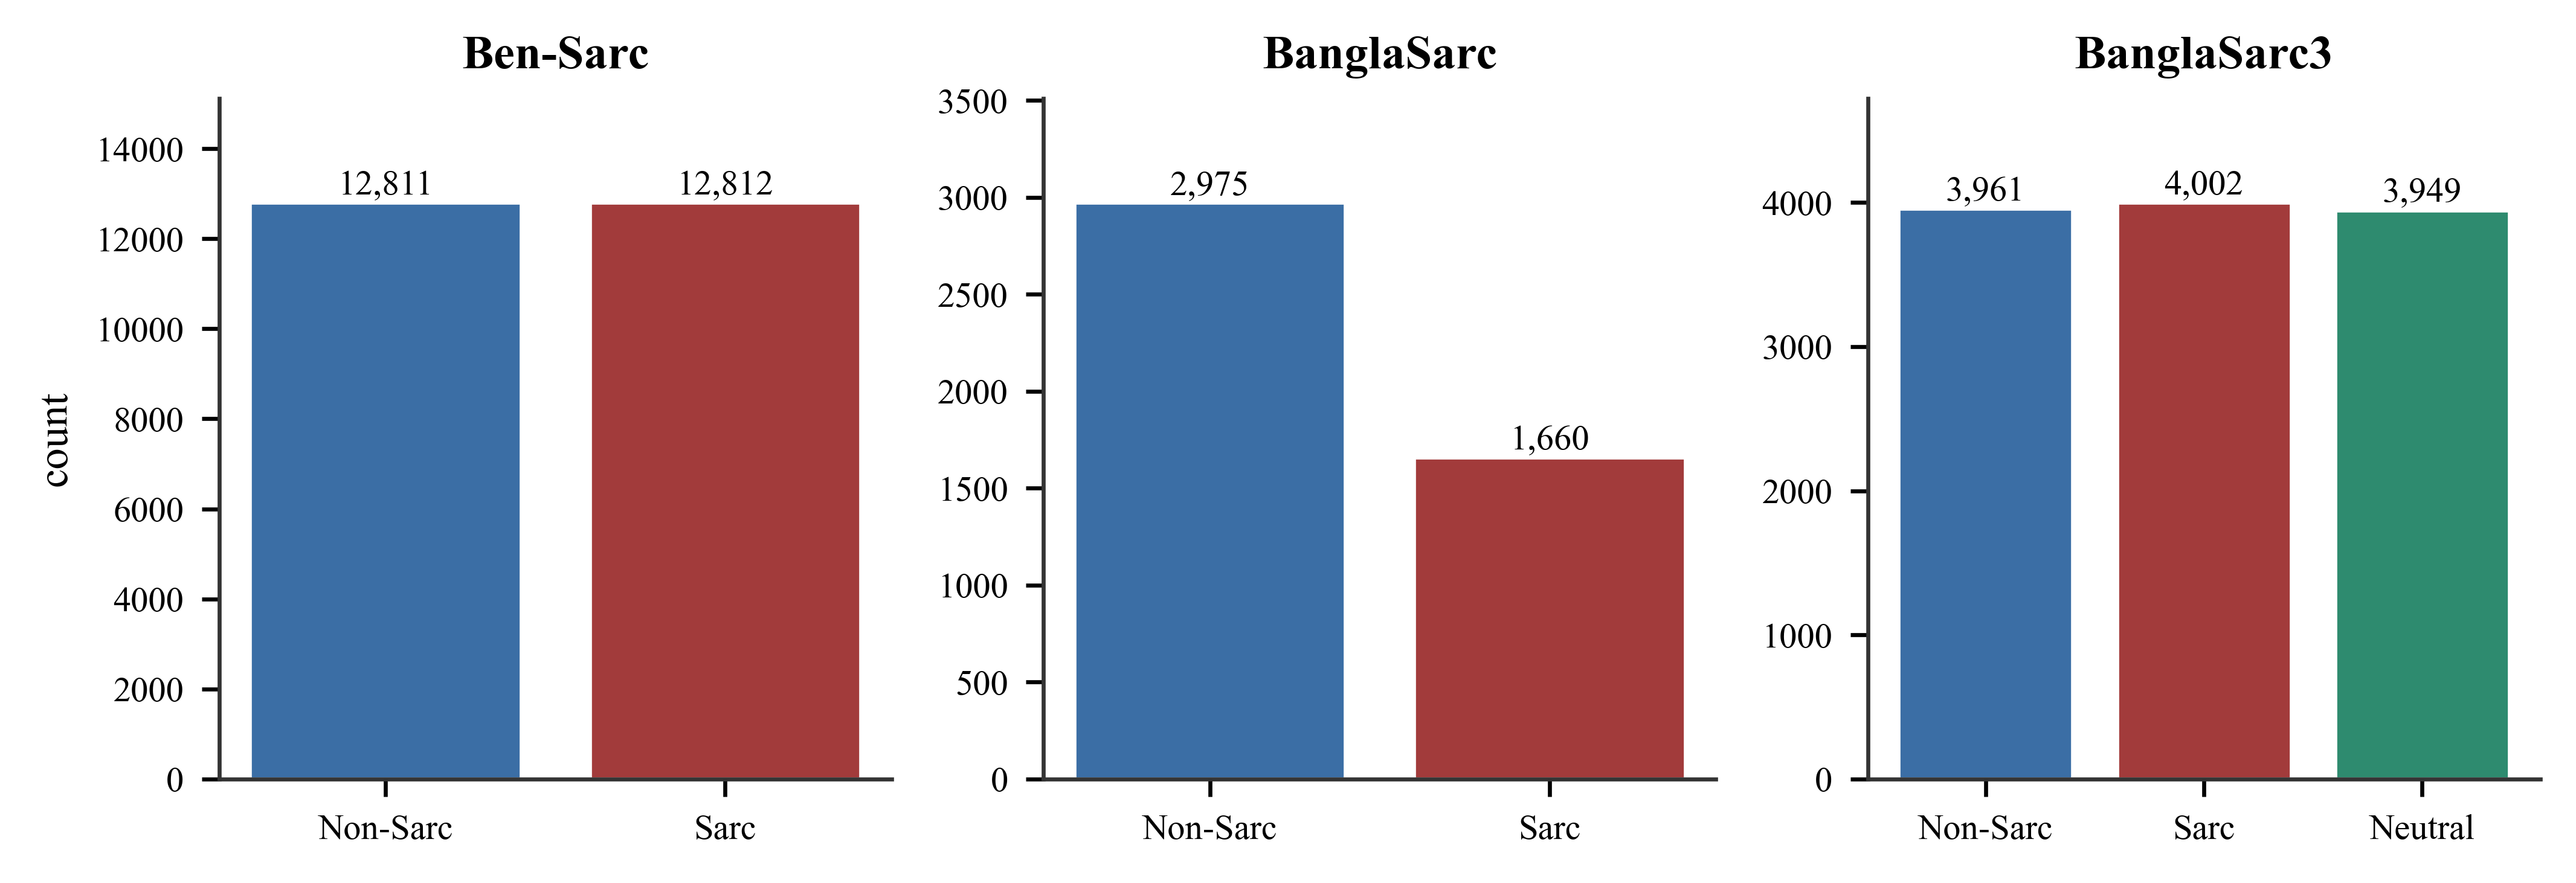
\includegraphics[width=0.98\columnwidth]{F_class_distribution.png}
\caption{Cleaned class distribution of the three corpora. \dset{Ben-Sarc} is balanced by construction, \dset{BanglaSarc} is imbalanced at roughly 36:64 sarcastic to non-sarcastic, and \dset{BanglaSarc3} carries a neutral class of comparable size to the other two.}
\label{fig:class-dist}
\end{figure}

The three corpora arrive with inconsistent schemas, so a two-stage pass audits shapes, missing values, and label distributions and then rewrites each dataset to a common schema. The cleaned class balance of each corpus is shown in \cref{fig:class-dist}. After ingest, we apply no additional lowercasing, punctuation stripping, diacritic removal, stemming, or stop-word removal. This statement concerns our pipeline; source repositories may already distribute cleaned text.

Deduplication is handled separately and, critically, \emph{before} any split is drawn. Define a normalization map $\nu:\mathcal{X}\to\mathcal{K}$ composing Unicode normalization form C (NFC), zero-width-character removal, whitespace collapse, and case-folding, and call $\nu(x)$ the key of comment $x$. Two comments share a key when they are identical after this normalization, so the procedure is normalized exact-match deduplication; it removes copies that differ only in spacing, case, or invisible characters, but not genuine near-duplicates that differ by a word substitution, an emoji, or an added clause. We retain one representative per key, drop rows whose duplicates disagree on the label, and then require of the partition $\{\mathcal{D}_{\mathrm{tr}},\mathcal{D}_{\mathrm{va}},\mathcal{D}_{\mathrm{te}}\}$ that
\begin{equation}
\nu(\mathcal{D}_{a})\,\cap\,\nu(\mathcal{D}_{b}) \;=\; \varnothing,
\quad a \neq b, \quad a,b \in \{\mathrm{tr},\mathrm{va},\mathrm{te}\}.
\label{eq:leakage-assertion}
\end{equation}
The assertion in \cref{eq:leakage-assertion} is re-run after every reload, so a comment cannot silently reappear across partitions when a downstream notebook reads the splits back from disk. Cleaning removed 9 normalized-exact copies and 4 label-conflicting rows from \dset{Ben-Sarc} (25{,}636 $\rightarrow$ 25{,}623), 477 duplicates from \dset{BanglaSarc} (5{,}112 $\rightarrow$ 4{,}635), and 109 duplicates plus 52 conflicts from the 12{,}072-row local \dset{BanglaSarc3} snapshot (12{,}072 $\rightarrow$ 11{,}911). These counts do not allege that the dataset authors performed no cleaning: our normalization key can collapse variants that an upstream rule retained, and the 52 conflicts are groups that agree under our key but carry different released labels. Exact split sizes and positive rates are preserved in the split audit, and the release inventory records SHA-256 hashes for each published,
sanitized artifact. The tagged release therefore supports exact reproduction of our cleaned local snapshot, but not independent verification that this snapshot is identical to the publisher's 12,089-row release.\Cref{fig:dataset-pipeline} shows the pipeline.

The original dataset papers describe their own cleaning procedures, including duplicate handling in Ben-Sarc and BanglaSarc3. Our contribution is narrower: one auditable normalized-exact-match rule is applied consistently to all three local copies before splitting, followed by an executable disjointness assertion. BanglaSarc has the largest reduction under this rule (477 rows). This fact is reported as a data audit and is not used to infer the cause of its transfer behavior.

\begin{figure*}[!t]
\centering
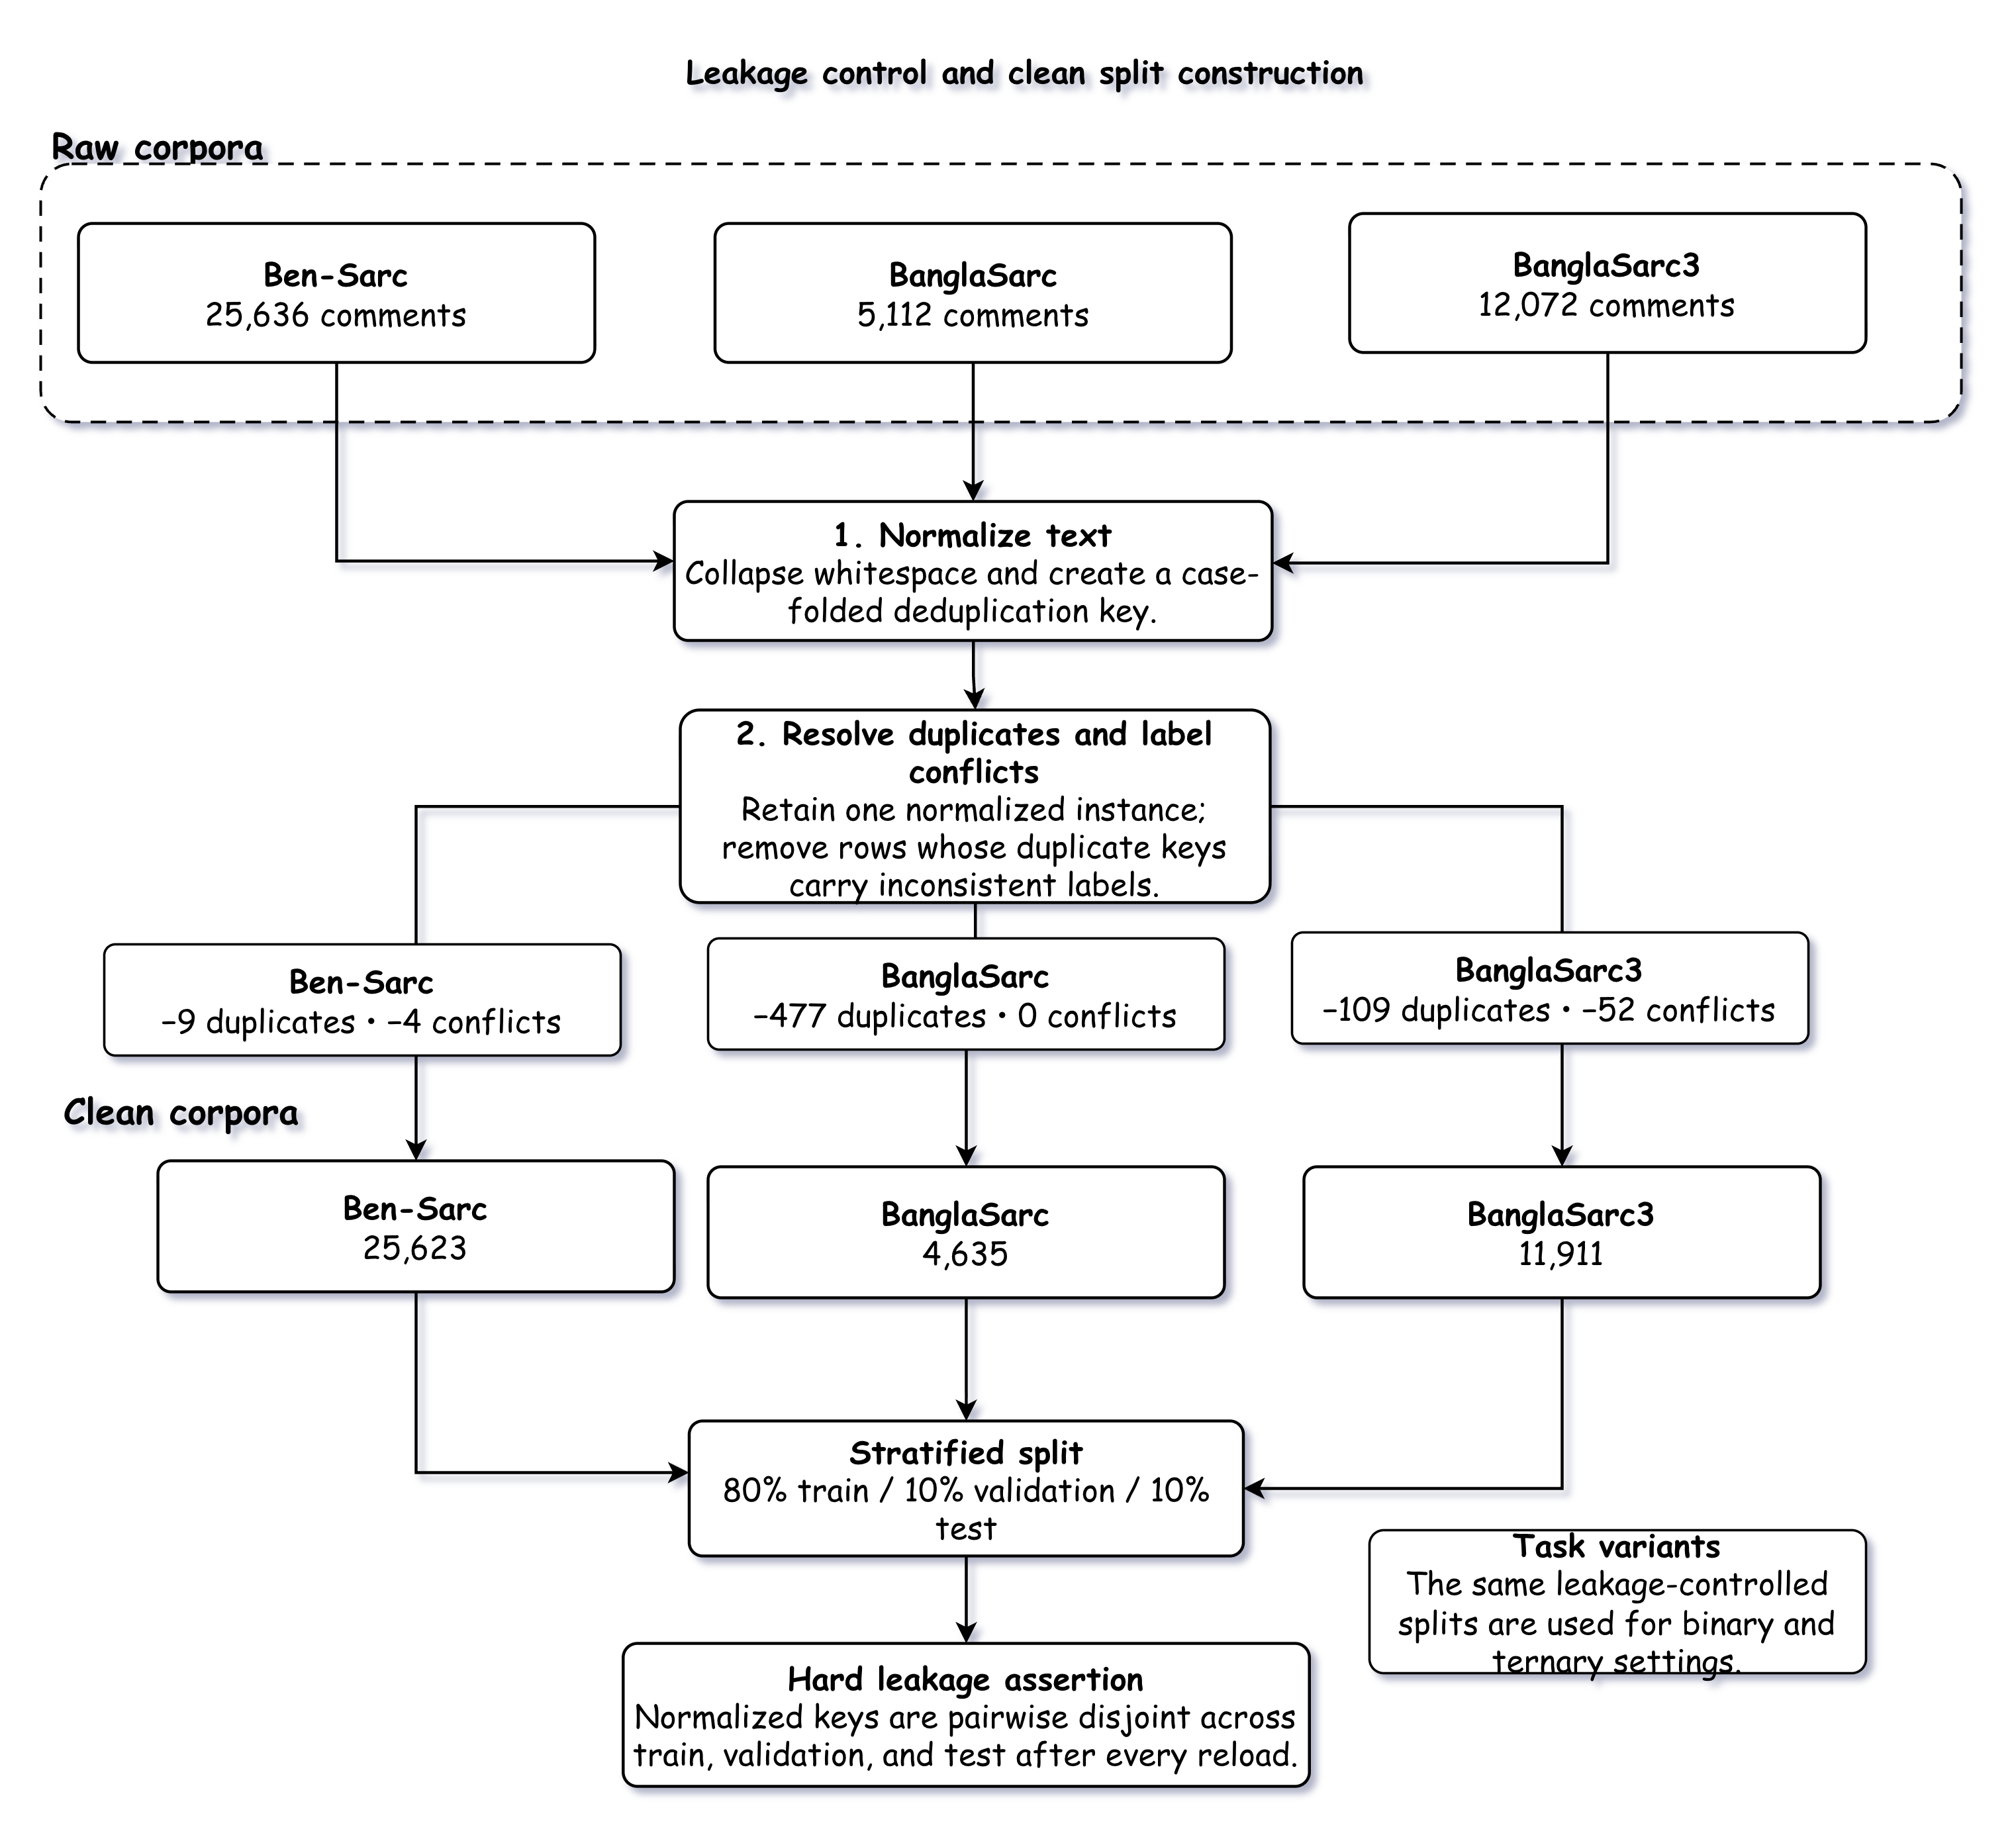
\includegraphics[width=\textwidth,height=0.36\textheight,keepaspectratio]{D2_data_leakage_control.png}
\caption{Data preparation and normalized-exact-match-controlled splitting. Raw corpora are audited, normalized, deduplicated on the key $\nu(x)$ with exact duplicates and label-conflicting rows dropped, then partitioned into seed-42 stratified 80/10/10 splits under the hard assertion of \cref{eq:leakage-assertion}. The same splits feed every downstream experiment.}
\label{fig:dataset-pipeline}
\end{figure*}

Four task variants follow: \dset{Ben-Sarc} binary (primary, 25{,}623 items), \dset{BanglaSarc} binary (4{,}635), \dset{BanglaSarc3} binary with the neutral class dropped (7{,}910), and \dset{BanglaSarc3} ternary (11{,}911). Each is partitioned by stratified sampling at 80/10/10, giving 20{,}498 / 2{,}562 / 2{,}563 on \dset{Ben-Sarc}, 3{,}708 / 463 / 464 on \dset{BanglaSarc}, 6{,}328 / 791 / 791 on \dset{BanglaSarc3} binary, and 9{,}528 / 1{,}191 / 1{,}192 on \dset{BanglaSarc3} ternary. Stratification preserves the class marginal, so that for every partition $\mathcal{P}$ and class $c$,
\begin{equation}
\frac{1}{|\mathcal{P}|}\sum_{i\in\mathcal{P}}\mathbb{1}[y_i = c] \;\approx\; \frac{n_c}{N},
\label{eq:stratified}
\end{equation}
which keeps the imbalanced corpora comparable across splits. The split seed is pinned at 42 throughout, so every model sees the same partitions. \Cref{tab:split-audit} reports the per-split sizes and sarcastic-class rates for the three repeated binary tasks. Checkpoint selection follows the validation-only criterion encoded in each saved notebook; some supporting notebooks use validation loss and others validation macro-F1. Test data are never used for checkpoint choice. Macro-F1 is primary, with accuracy alongside for continuity with the reference paper.

\begin{table}[!t]
\centering
\caption{Notebook 18 split audit for the three repeated binary tasks. Rates denote the sarcastic class.}
\label{tab:split-audit}
\footnotesize
\setlength{\tabcolsep}{3pt}
\begin{tabular}{@{}lrrr@{}}
\toprule
\textbf{Corpus} & \textbf{Train} & \textbf{Validation} & \textbf{Test} \\
\midrule
Ben-Sarc & 20{,}498 (0.500) & 2{,}562 (0.500) & 2{,}563 (0.500) \\
BanglaSarc & 3{,}708 (0.358) & 463 (0.359) & 464 (0.358) \\
BanglaSarc3 & 6{,}328 (0.499) & 791 (0.499) & 791 (0.499) \\
\bottomrule
\end{tabular}
\end{table}


\section{Methodology}
\label{sec:methodology}

The contribution is an evaluation framework, not a new architecture or a domain-adaptation method. All tracks use the partitions in \cref{sec:dataset-cleaning-and-splits}. The reproduction track reruns classical, recurrent, and frozen-encoder families on Ben-Sarc. The in-domain benchmark compares five encoders using their native sequence-classification heads under a standardized training budget. The generalization track estimates unadapted cross-corpus transfer; adversarial methods and ensembles remain secondary analyses. Pooled or leave-one-corpus-out training would answer the distinct mitigation question and is reserved for future work.

\subsection{Full Fine-Tuning and Evaluated Configurations}
\label{sec:proposed-architecture}

For the primary BanglaBERT system, classification is represented as a linear map of the sequence representation,
\begin{equation}
\mathbf{z} = \mathbf{W}_c\,\mathbf{h}_{[CLS]} + \mathbf{b}_c,\qquad
\hat{p}(y\!\mid\!x;\theta,\phi) = \mathrm{softmax}(\mathbf{z}),
\label{eq:classifier}
\end{equation}
trained by minimizing the empirical cross-entropy
\begin{equation}
\mathcal{L}_{CE}(\theta,\phi) = -\frac{1}{N}\sum_{i=1}^{N}\sum_{c=1}^{C}y_{i,c}\,\log\hat{p}\!\left(y\!=\!c\mid x_i;\theta,\phi\right).
\label{eq:ce}
\end{equation}
Unlike the frozen reference systems, we jointly optimize encoder parameters $\theta$ and head parameters $\phi$ with AdamW \cite{loshchilov2019adamw}. The standardized multi-backbone comparison uses each library checkpoint's native sequence-classification head, documented in \cref{sec:phase-multibackbone}; \cref{eq:classifier} is not a claim that every model family's implementation is structurally identical. Two result streams must not be conflated. The \emph{primary repeated configuration} uses BanglaBERT's native classification head, maximum length 128, full fine-tuning, and FGM with $\epsilon=0.5$; it is repeated over five seeds. The \emph{exploratory enhanced configuration} is one seed-42 run with maximum length 192, layer-wise learning-rate decay, concatenated \texttt{[CLS]} and masked-mean pooling, a two-layer MLP, label smoothing $s=0.05$, FGM, and AWP. Its smoothed target is
\begin{equation}
\tilde{y}_{i,c} = (1-s)\,y_{i,c} + \frac{s}{C},
\label{eq:label-smoothing}
\end{equation}
and inverse-frequency weights are $w_c=N/(Cn_c)$. On balanced Ben-Sarc these weights equal one. The exploratory run accumulates clean, FGM, and AWP losses before each optimizer step and selects the minimum validation-loss checkpoint. Because it changes the head, length, optimizer schedule, loss, and adversarial procedure together and was run once, it is reported as a configuration-level observation rather than a causal ablation or a repeated headline estimate. \Cref{fig:proposed-model} depicts this enhanced configuration.

\begin{figure}[tb]
\centering
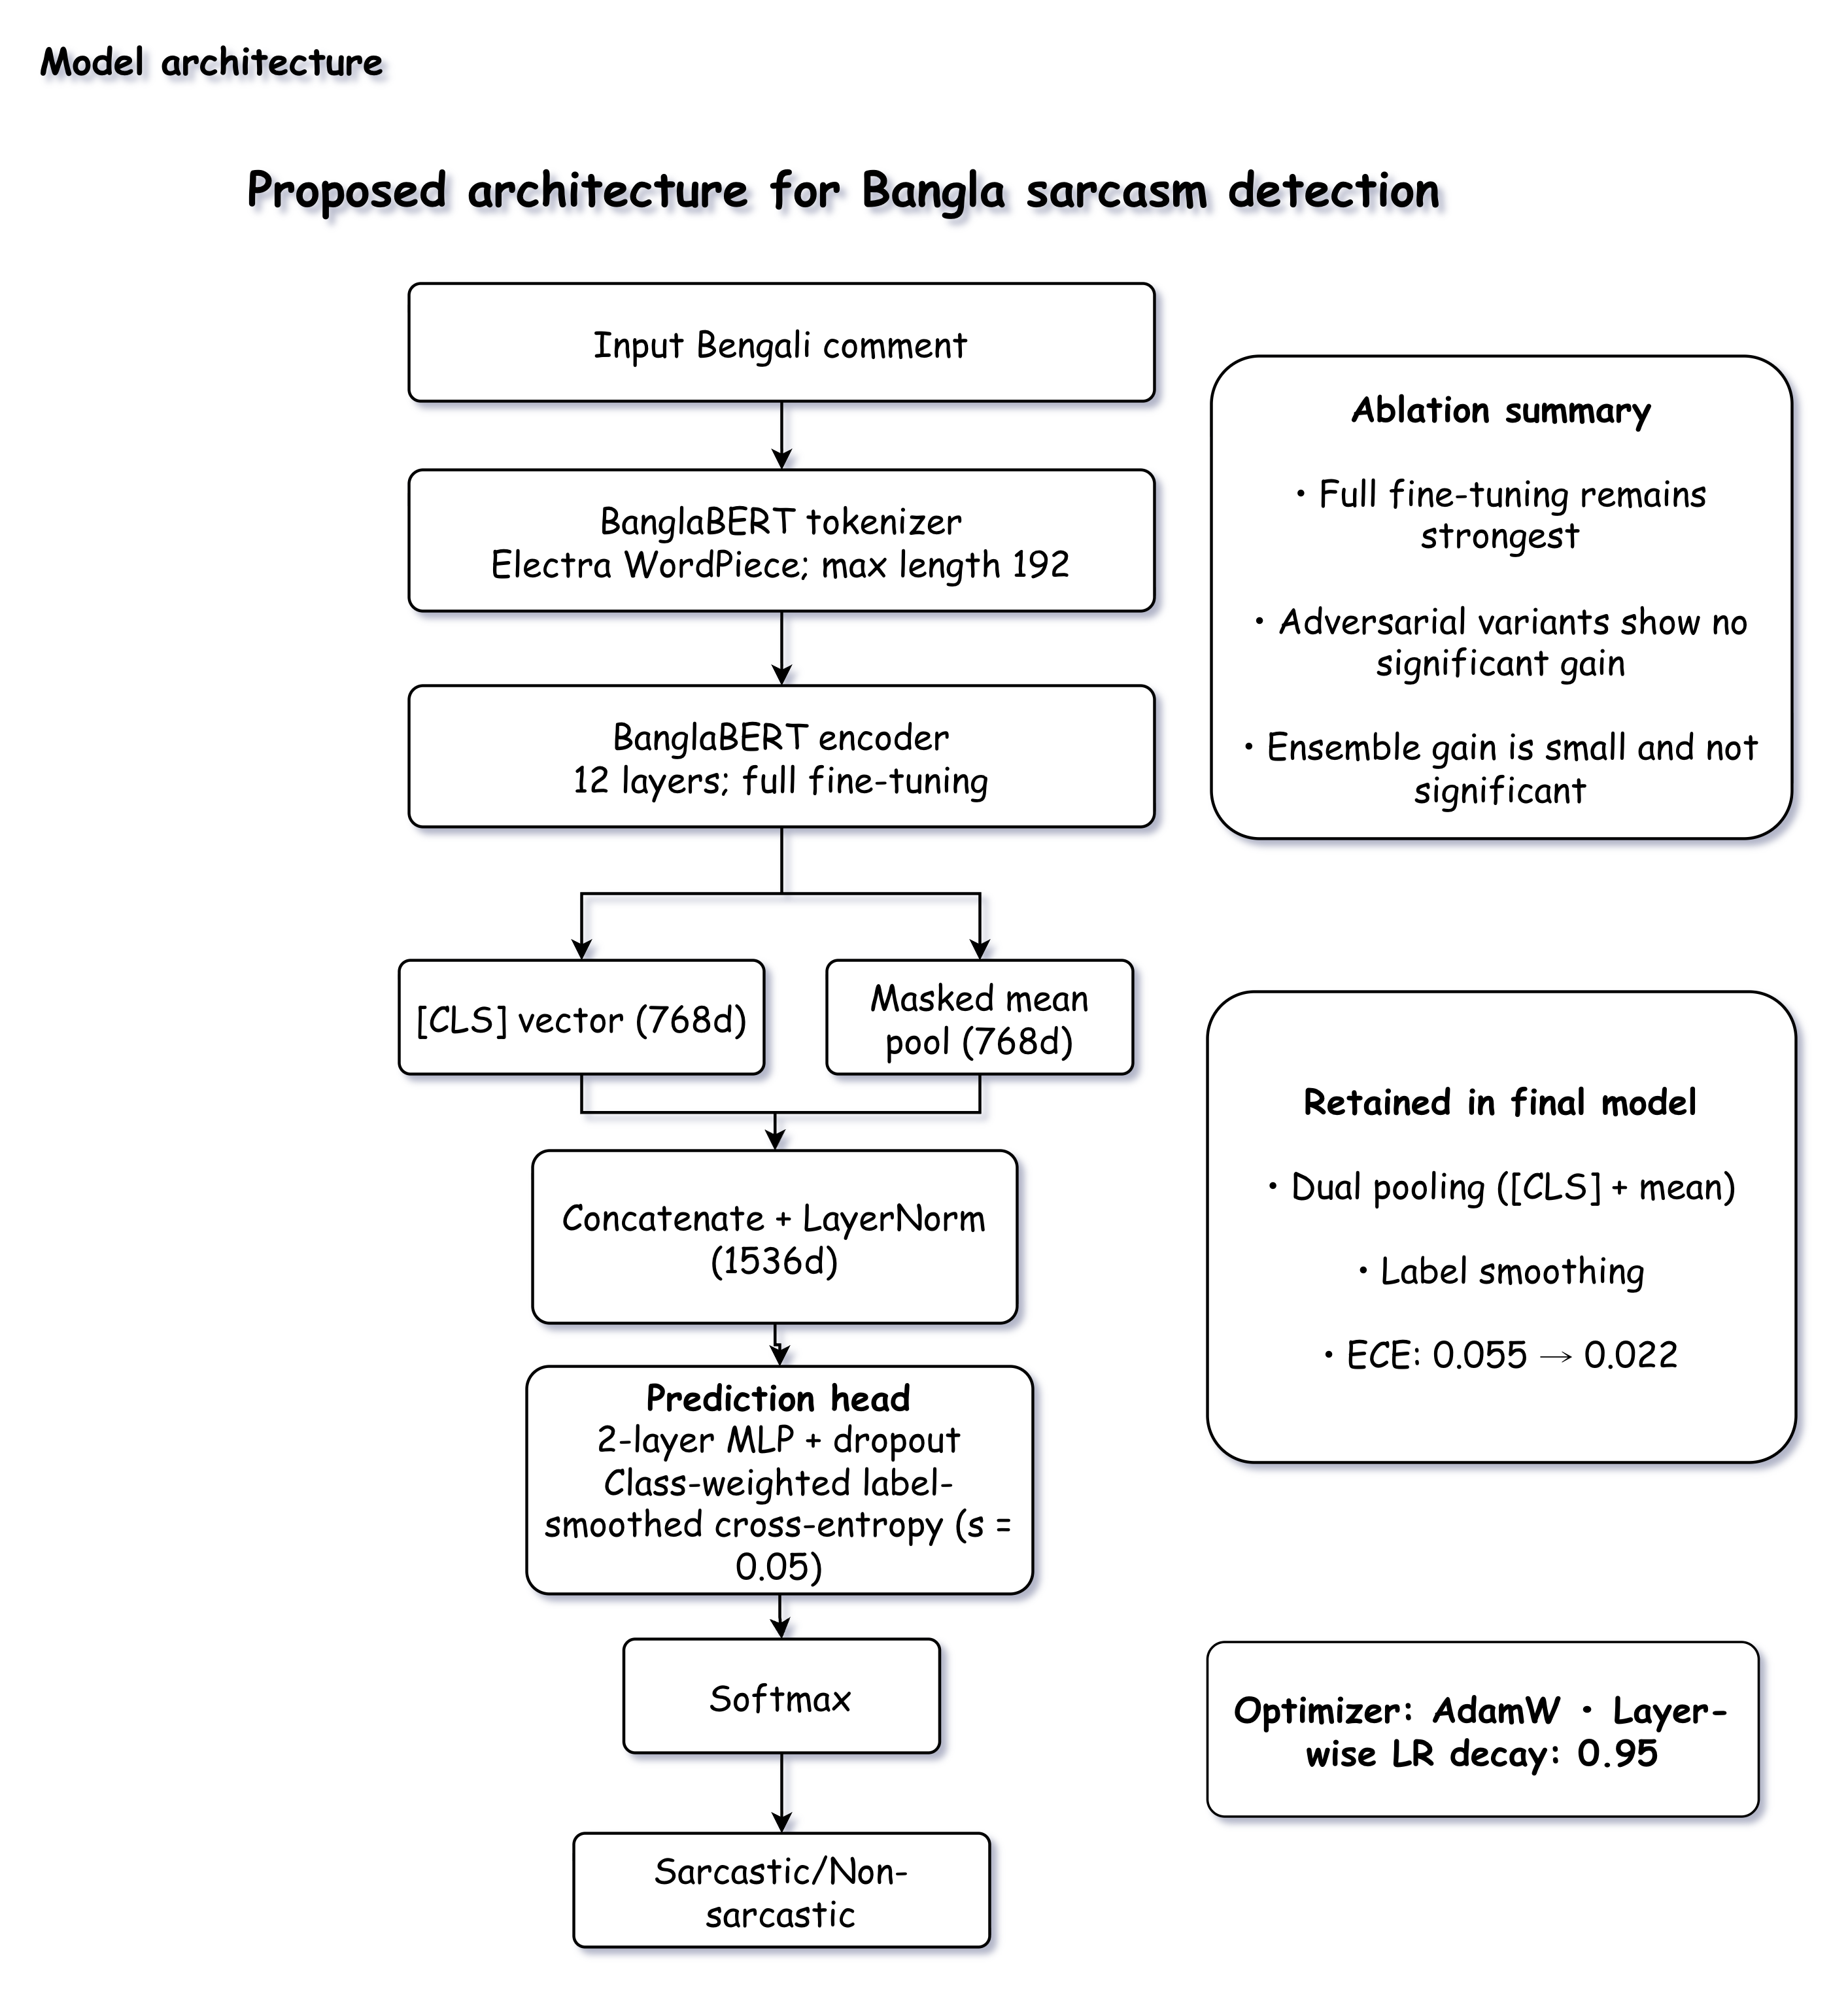
\includegraphics[width=0.76\columnwidth]{D4_proposed_model.png}
\caption{The exploratory enhanced configuration: BanglaBERT fine-tuned end-to-end with concatenated \texttt{[CLS]} and masked-mean pooling into a two-layer MLP head, trained with label smoothing, FGM, and AWP. It is a single seed-42 run, reported as a configuration-level observation rather than a repeated headline system.}
\label{fig:proposed-model}
\end{figure}
\begin{equation}
\mathcal{L}_{CE} = -\frac{1}{N}\sum_{i=1}^{N} w_{y_i}\sum_{c=1}^{C}\tilde{y}_{i,c}\,\log\hat{p}_{i,c}.
\label{eq:weighted-ls}
\end{equation}

\subsection{Multi-Backbone Benchmarking}
\label{sec:phase-multibackbone}

Five Bengali-capable encoders are compared under one standardized computational budget (\cref{tab:backbones}). The implementation requests a sequence-classification model from each checkpoint and uses its native classification head; those heads need not be structurally identical across model families. Splits, epoch budget, optimizer, and base learning rate are held fixed, but the absence of per-backbone tuning can favor some architectures. The experiment therefore measures performance under one common budget rather than isolating a causal encoder effect or establishing a definitive ranking. Exact model identifiers and the instantiated head classes are recorded in the backbone notebook and machine-readable configuration.

\begin{table}[!t]
\centering
\caption{Transformer backbones evaluated in this work.}
\label{tab:backbones}
\footnotesize
\setlength{\tabcolsep}{3pt}
\begin{tabularx}{\columnwidth}{@{}lrlX@{}}
\toprule
\textbf{Backbone} & \textbf{Params} & \textbf{Tokenizer} & \textbf{Pre-training corpus} \\
\midrule
BanglaBERT \cite{bhattacharjee2022banglabert} & 110M & WordPiece & 27.5\,GB Bengali, 110 sites (mono.) \\
MuRIL \cite{khanuja2021muril} & 236M & WordPiece & 17 Indian langs.\ + transliterated (multi.) \\
XLM-RoBERTa \cite{conneau2020xlmr} & 270M & SentencePiece & 2.5\,TB CommonCrawl, 100 langs. (multi.) \\
mBERT \cite{devlin2019bert} & 178M & WordPiece & Wikipedia, 102 langs. (multi.) \\
Sagorsarker BB & 110M & WordPiece & Bengali Wikipedia + OSCAR (mono.) \\
\bottomrule
\end{tabularx}
\end{table}

\subsection{Cross-Corpus Transfer Evaluation}
\label{sec:phase-crossdataset}

A model trained on one Bengali sarcasm corpus is not automatically a model that works on another, and the only way to find out is to try. We build a zero-shot transfer matrix $\mathbf{M}\in\mathbb{R}^{3\times3}$ over the three binary corpora, with entries
\begin{equation}
M_{jk} \;=\; \mathrm{macro\text{-}F1}\!\left(f_{\mathcal{D}_j},\, \widetilde{\mathcal{D}}_{k,\mathrm{te}}\right),
\label{eq:transfer-matrix}
\end{equation}
\begin{equation}
\widetilde{\mathcal{D}}_{k,\mathrm{te}} \;=\; \bigl\{(x,y)\in\mathcal{D}_{k,\mathrm{te}} \;:\; \nu(x)\notin\nu(\mathcal{D}_{j,\mathrm{all}})\bigr\},
\label{eq:transfer-filter}
\end{equation}
where $f_{\mathcal{D}_j}$ is a BanglaBERT classifier trained only on the training split of corpus $j$, while $\mathcal{D}_{j,\mathrm{all}}=\mathcal{D}_{j,\mathrm{tr}}\cup\mathcal{D}_{j,\mathrm{va}}\cup\mathcal{D}_{j,\mathrm{te}}$ is used \emph{only} for overlap auditing. This conservative filter removes a target-test comment if its normalized key appears anywhere in the source corpus, even if that source item was never used to optimize the model. Diagonal entries $M_{jj}$ are in-domain; off-diagonal entries are direct zero-shot transfer. \Cref{fig:transfer-protocol} summarizes the protocol.

\begin{figure*}[t]
\centering
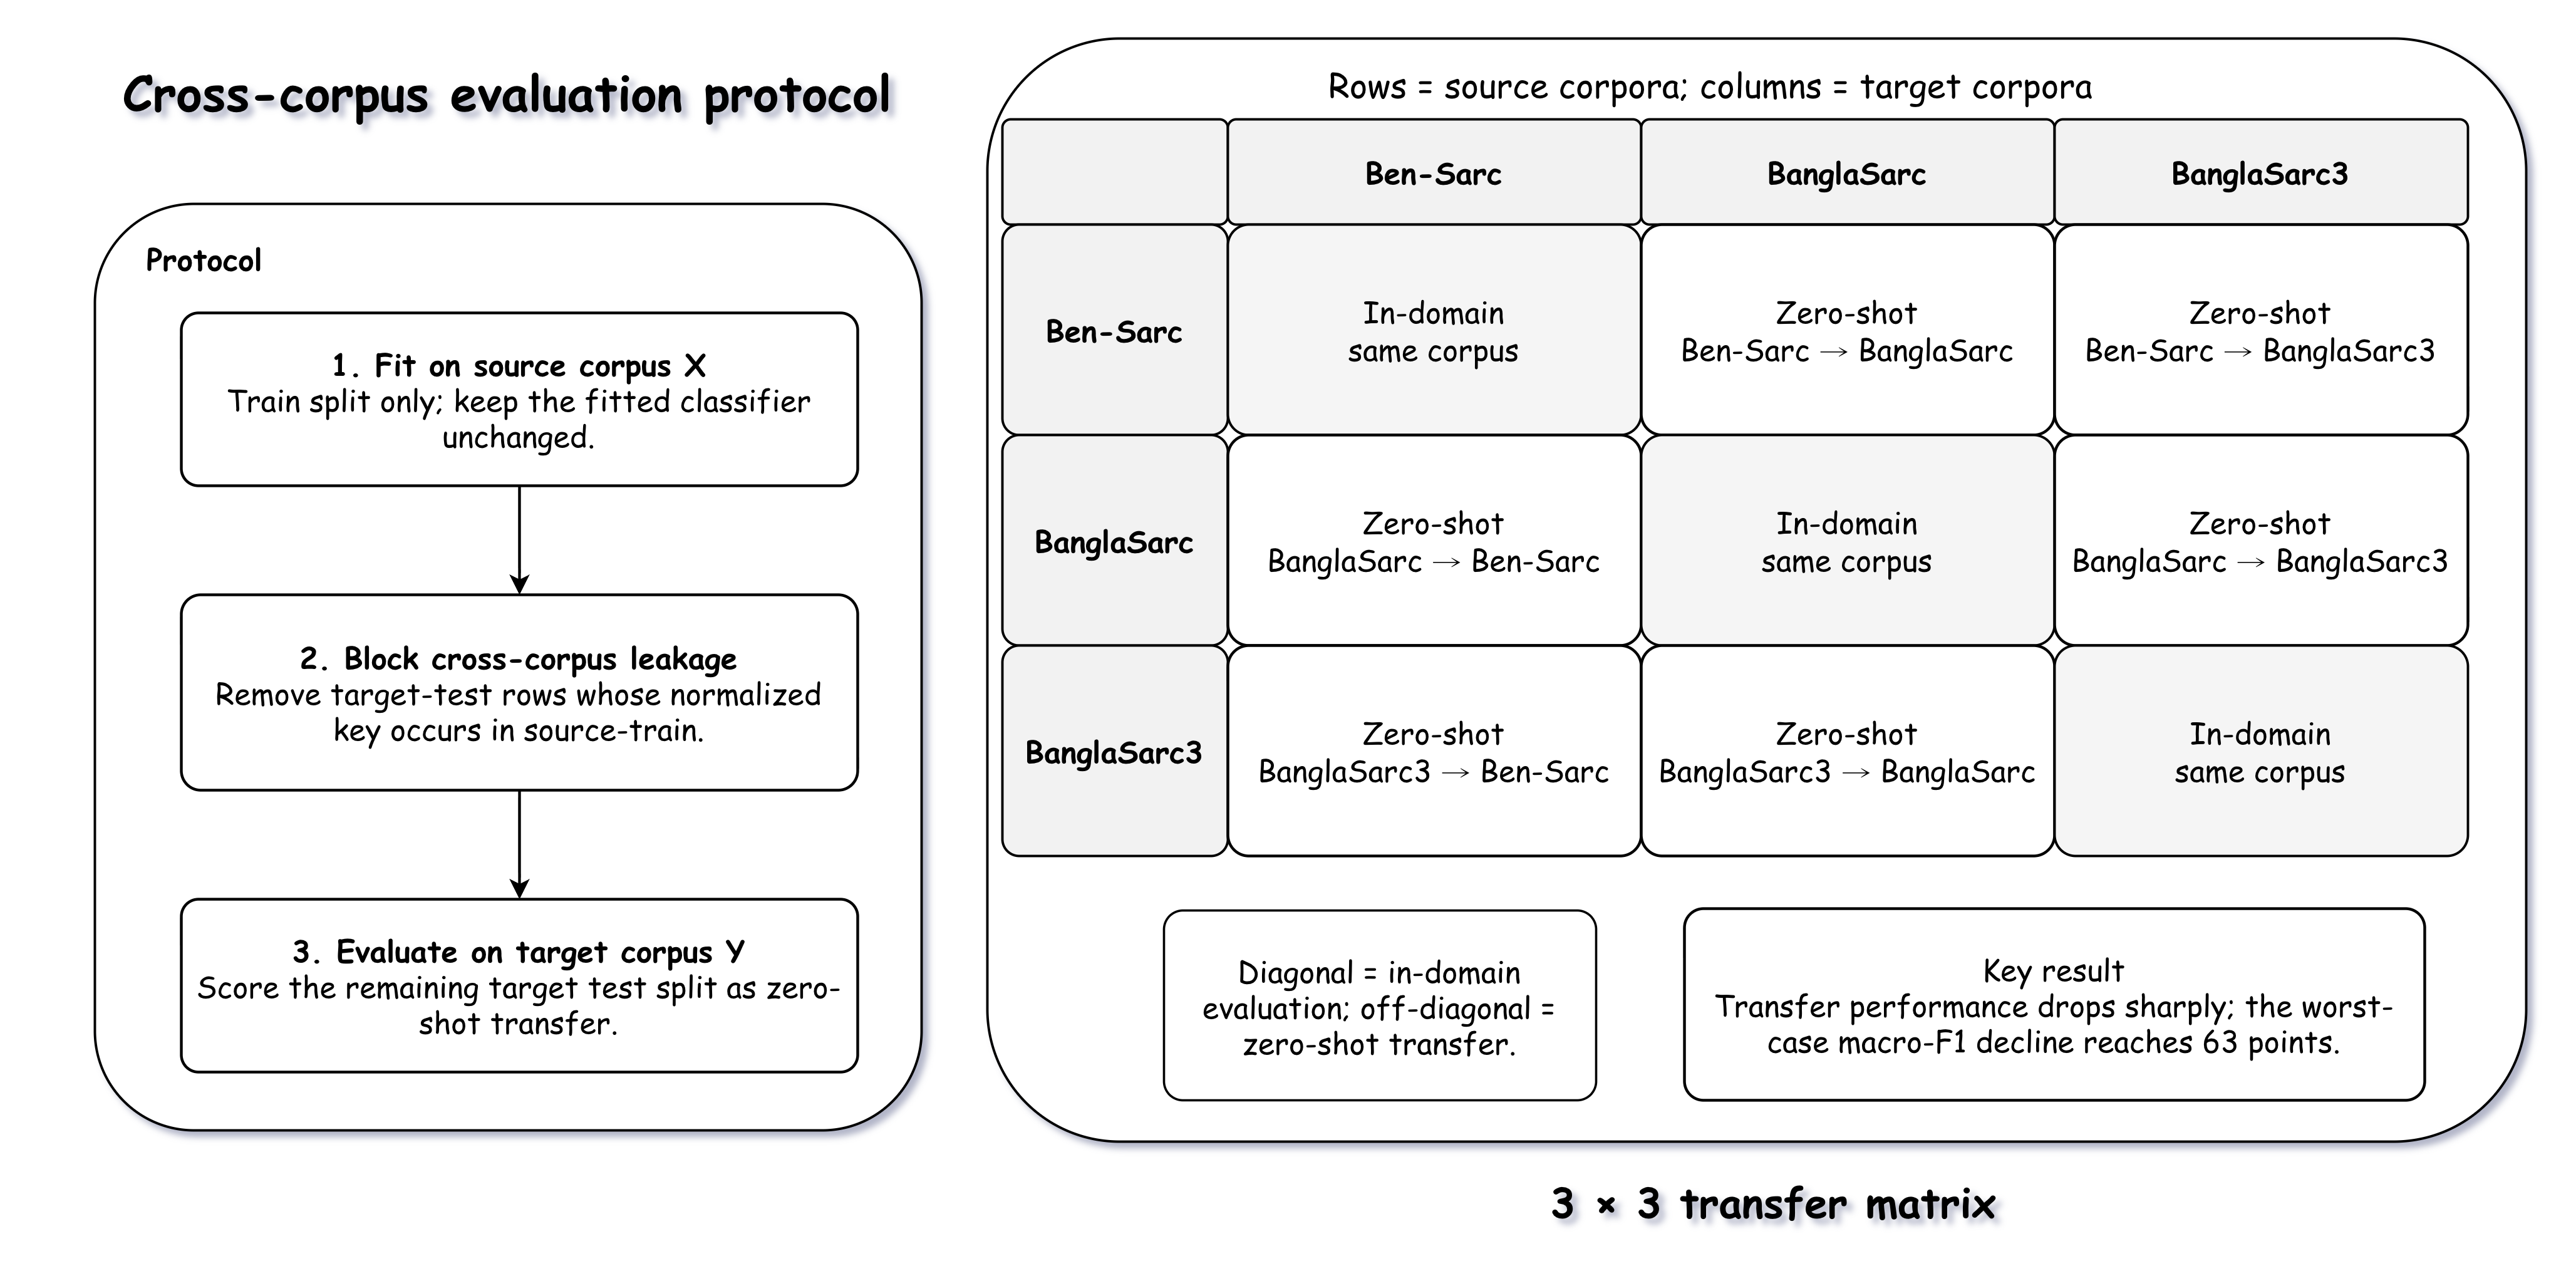
\includegraphics[width=\textwidth,height=0.26\textheight,keepaspectratio]{D3_cross_corpus_protocol.png}
\caption{Cross-corpus evaluation protocol. Each source-trained model is scored on every target test split after removing any target comment whose normalized key $\nu(x)$ appears anywhere in the source corpus (train, validation, or test); diagonal cells are in-domain and off-diagonal cells are unadapted zero-shot transfer between corpus-specific operational labelings. No target-corpus fine-tuning or adaptation is performed.}
\label{fig:transfer-protocol}
\end{figure*}

The authoritative experiment instantiates \cref{eq:transfer-matrix} for two systems $a\in\{\mathrm{vanilla},\mathrm{FGM}\}$ and five matched seeds $s\in\{42,1,7,123,2024\}$, producing
\begin{equation}
M^{(a,s)}_{jk}=\mathrm{macro\text{-}F1}\!\left(f^{(a,s)}_{\mathcal D_j},\widetilde{\mathcal D}_{k,\mathrm{te}}\right).
\label{eq:repeated-transfer}
\end{equation}
Thus the primary design trains $2\times3\times5=30$ models. Evaluating every trained model on three targets produces $30\times3=90$ source--target evaluation cells; a target evaluation is not a separate training run. For each fixed system and source--target pair, we report the five-seed mean, sample standard deviation, and two-sided Student-$t$ 95\% confidence interval. The older single-seed transfer output is retained only as provenance and is superseded by \cref{eq:repeated-transfer} for all headline claims.

To summarize a row, define the generalization gap of corpus $j$ as the distance between its in-domain score and its mean transfer score,
\begin{equation}
\Gamma(\mathcal{D}_j) \;=\; M_{jj} \;-\; \frac{1}{|\mathcal{J}|-1}\sum_{k\neq j} M_{jk},
\label{eq:gap}
\end{equation}
which is zero for a classifier whose outgoing score equals its source-domain score. Because $\Gamma$ also reflects target difficulty, we additionally report target-relative loss and retention,
\begin{equation}
L_{j\rightarrow k}=M_{kk}-M_{jk},\qquad
R_{j\rightarrow k}=\frac{M_{jk}}{M_{kk}},\quad j\neq k,
\label{eq:target-relative}
\end{equation}
where the transferred model is compared with a model trained on the target corpus under the same system. These are descriptive comparisons, not causal decompositions of domain shift. No fine-tuning, domain adaptation, or self-training is performed on the target corpus, since the question is how much target-trained performance survives when training data come from another corpus; any adaptation would answer a different question.

The primary filter in \cref{eq:transfer-filter} is pair-specific and therefore changes the test population for two directed cells. We consequently define a source-independent sensitivity population directly from the corpus keys,
\begin{equation}
\mathcal D^{\mathrm{fixed}}_{k,\mathrm{te}}=
\bigl\{(x,y)\in\mathcal D_{k,\mathrm{te}}:\nu(x)\notin
\bigcup_{j\ne k}\nu(\mathcal D_{j,\mathrm{all}})\bigr\}.
\label{eq:fixed-target}
\end{equation}
This yields 2{,}563 Ben-Sarc, 436 BanglaSarc, and 762 BanglaSarc3 comments. It is determined from hashed split manifests, independently of model or prediction availability. As a reproducibility check, these three sets are identical to the intersections recovered from all 90 saved prediction files. The fixed-target metrics require only rescoring existing predictions, not retraining. For each system, directed pair, and matched seed, \cref{eq:target-relative} is evaluated on the same fixed target items before computing its mean, standard deviation, and Student-$t$ 95\% interval.


\subsection{Adversarial Training (Ablation)}
\label{sec:adv-framework}

The matched adversarial experiment holds BanglaBERT's native head and seed fixed and evaluates FGM, FreeLB, AWP, and FGM+AWP. For FGM, the embedding perturbation is
\begin{equation}
\mathbf{r}_{\mathrm{adv}}=\epsilon\frac{\nabla_{\mathbf e}\mathcal L_{CE}}{\|\nabla_{\mathbf e}\mathcal L_{CE}\|_2},
\label{eq:fgm-radv}
\end{equation}
with $\epsilon=0.5$ selected from $\{0.1,0.3,0.5,1.0\}$ by validation macro-F1. FreeLB uses three projected inner steps. AWP perturbs eligible weights with relative scale $\alpha=0.01$, clipping $10^{-3}$, and begins after epoch 1 \cite{wu2020awp}. These are exploratory single-seed ablations. The separate enhanced run combines FGM and AWP with the additional changes described above, so its score cannot isolate an adversarial-training effect.

\section{Reproduction Pipeline and Experimental Setup}
\label{sec:setup}

\subsection{Why Reproduction Matters}
\label{sec:why-repro}

Comparing our model against the numbers printed in Lora et al.\ \cite{lora2025bensarc} would not test anything. Their numbers come from different splits and different preprocessing, so a difference between a published score and ours confounds the method effect with split and protocol effects, and no amount of care afterward can separate them. The reproduction track removes the principal split confound by reimplementing each of the three reference method families on our fixed, normalized-exact-match-controlled splits under the same metric and the same tests. The target is protocol-faithful reproduction rather than a bit-exact match, which is rarely achievable even for well-documented systems. Where reproduced numbers disagree with published ones, \cref{sec:negative-results} says so.

\subsection{Reproduced Baselines}
\label{sec:reproduced-baselines}

\runin{Traditional machine learning.} The seven classical classifiers of Lora et al.\ \cite{lora2025bensarc} are reproduced: logistic regression, decision tree, random forest, multinomial naive Bayes, $k$-nearest neighbors, linear support vector machine (SVM), and kernel SVM. Each is paired with TF-IDF features over unigrams, bigrams, and trigrams, where the weight of term $t$ in document $q$ is
\begin{equation}
\mathrm{tfidf}(t,q) \;=\; \mathrm{tf}(t,q)\cdot\left(\log\frac{1+N}{1+\mathrm{df}(t)} + 1\right),
\label{eq:tfidf}
\end{equation}
with $\mathrm{df}(t)$ the document frequency, after which each document vector is $\ell_2$-normalized. The $n$-gram setting maximizing cross-validation macro-F1 is carried into the test evaluation per classifier, which isolates the choice of $n$ from the choice of model. The strongest reproduced classical system on \dset{Ben-Sarc} binary is multinomial naive Bayes with trigram TF-IDF at 0.6602 macro-F1, with kernel SVM a thousandth behind (\cref{fig:classical-ml}).

\runin{Deep learning.} Six recurrent and recurrent-convolutional architectures are reproduced: LSTM, LSTM+CNN, LSTM+\allowbreak CNN+\allowbreak GloVe, stacked LSTM+\allowbreak CNN+\allowbreak GloVe, BiLSTM+\allowbreak CNN+\allowbreak GloVe, and BiLSTM+\allowbreak GloVe. The GloVe variants use the same Bengali global-vectors embeddings as the reference paper (300-dimensional, frozen); the rest learn embeddings from scratch. Training uses binary cross-entropy with early stopping on validation loss. The strongest reproduced deep model is BiLSTM+GloVe at 0.7127 macro-F1. On the clean split the GloVe variants exceed the published numbers while the from-scratch models land within about 1.5 points of them, which is the expected signature of a faithful but not identical reproduction; the per-model comparison is available in the public code repository.

\runin{Frozen-encoder transfer.} The reference paper used three frozen encoders: BanglaBERT (Sagorsarker), mBERT, and Indic-Transformers Bengali BERT, the last being their strongest at 75.05\% accuracy. The first two reproduce under a seven-dense-layer frozen head, reaching 0.6921 and 0.6916 macro-F1. The third checkpoint, \texttt{neuralspace\-reverie/\allowbreak indic\-transformers\-bn\-bert}, could not be retrieved. We therefore evaluate \texttt{l3cube\-pune/bengali\-bert} under the same protocol; it reaches 0.7444 macro-F1. This is an explicit substitute, not a reproduction of the unavailable checkpoint, and all paired claims are limited to its saved predictions.

\begin{figure}[!t]
\centering
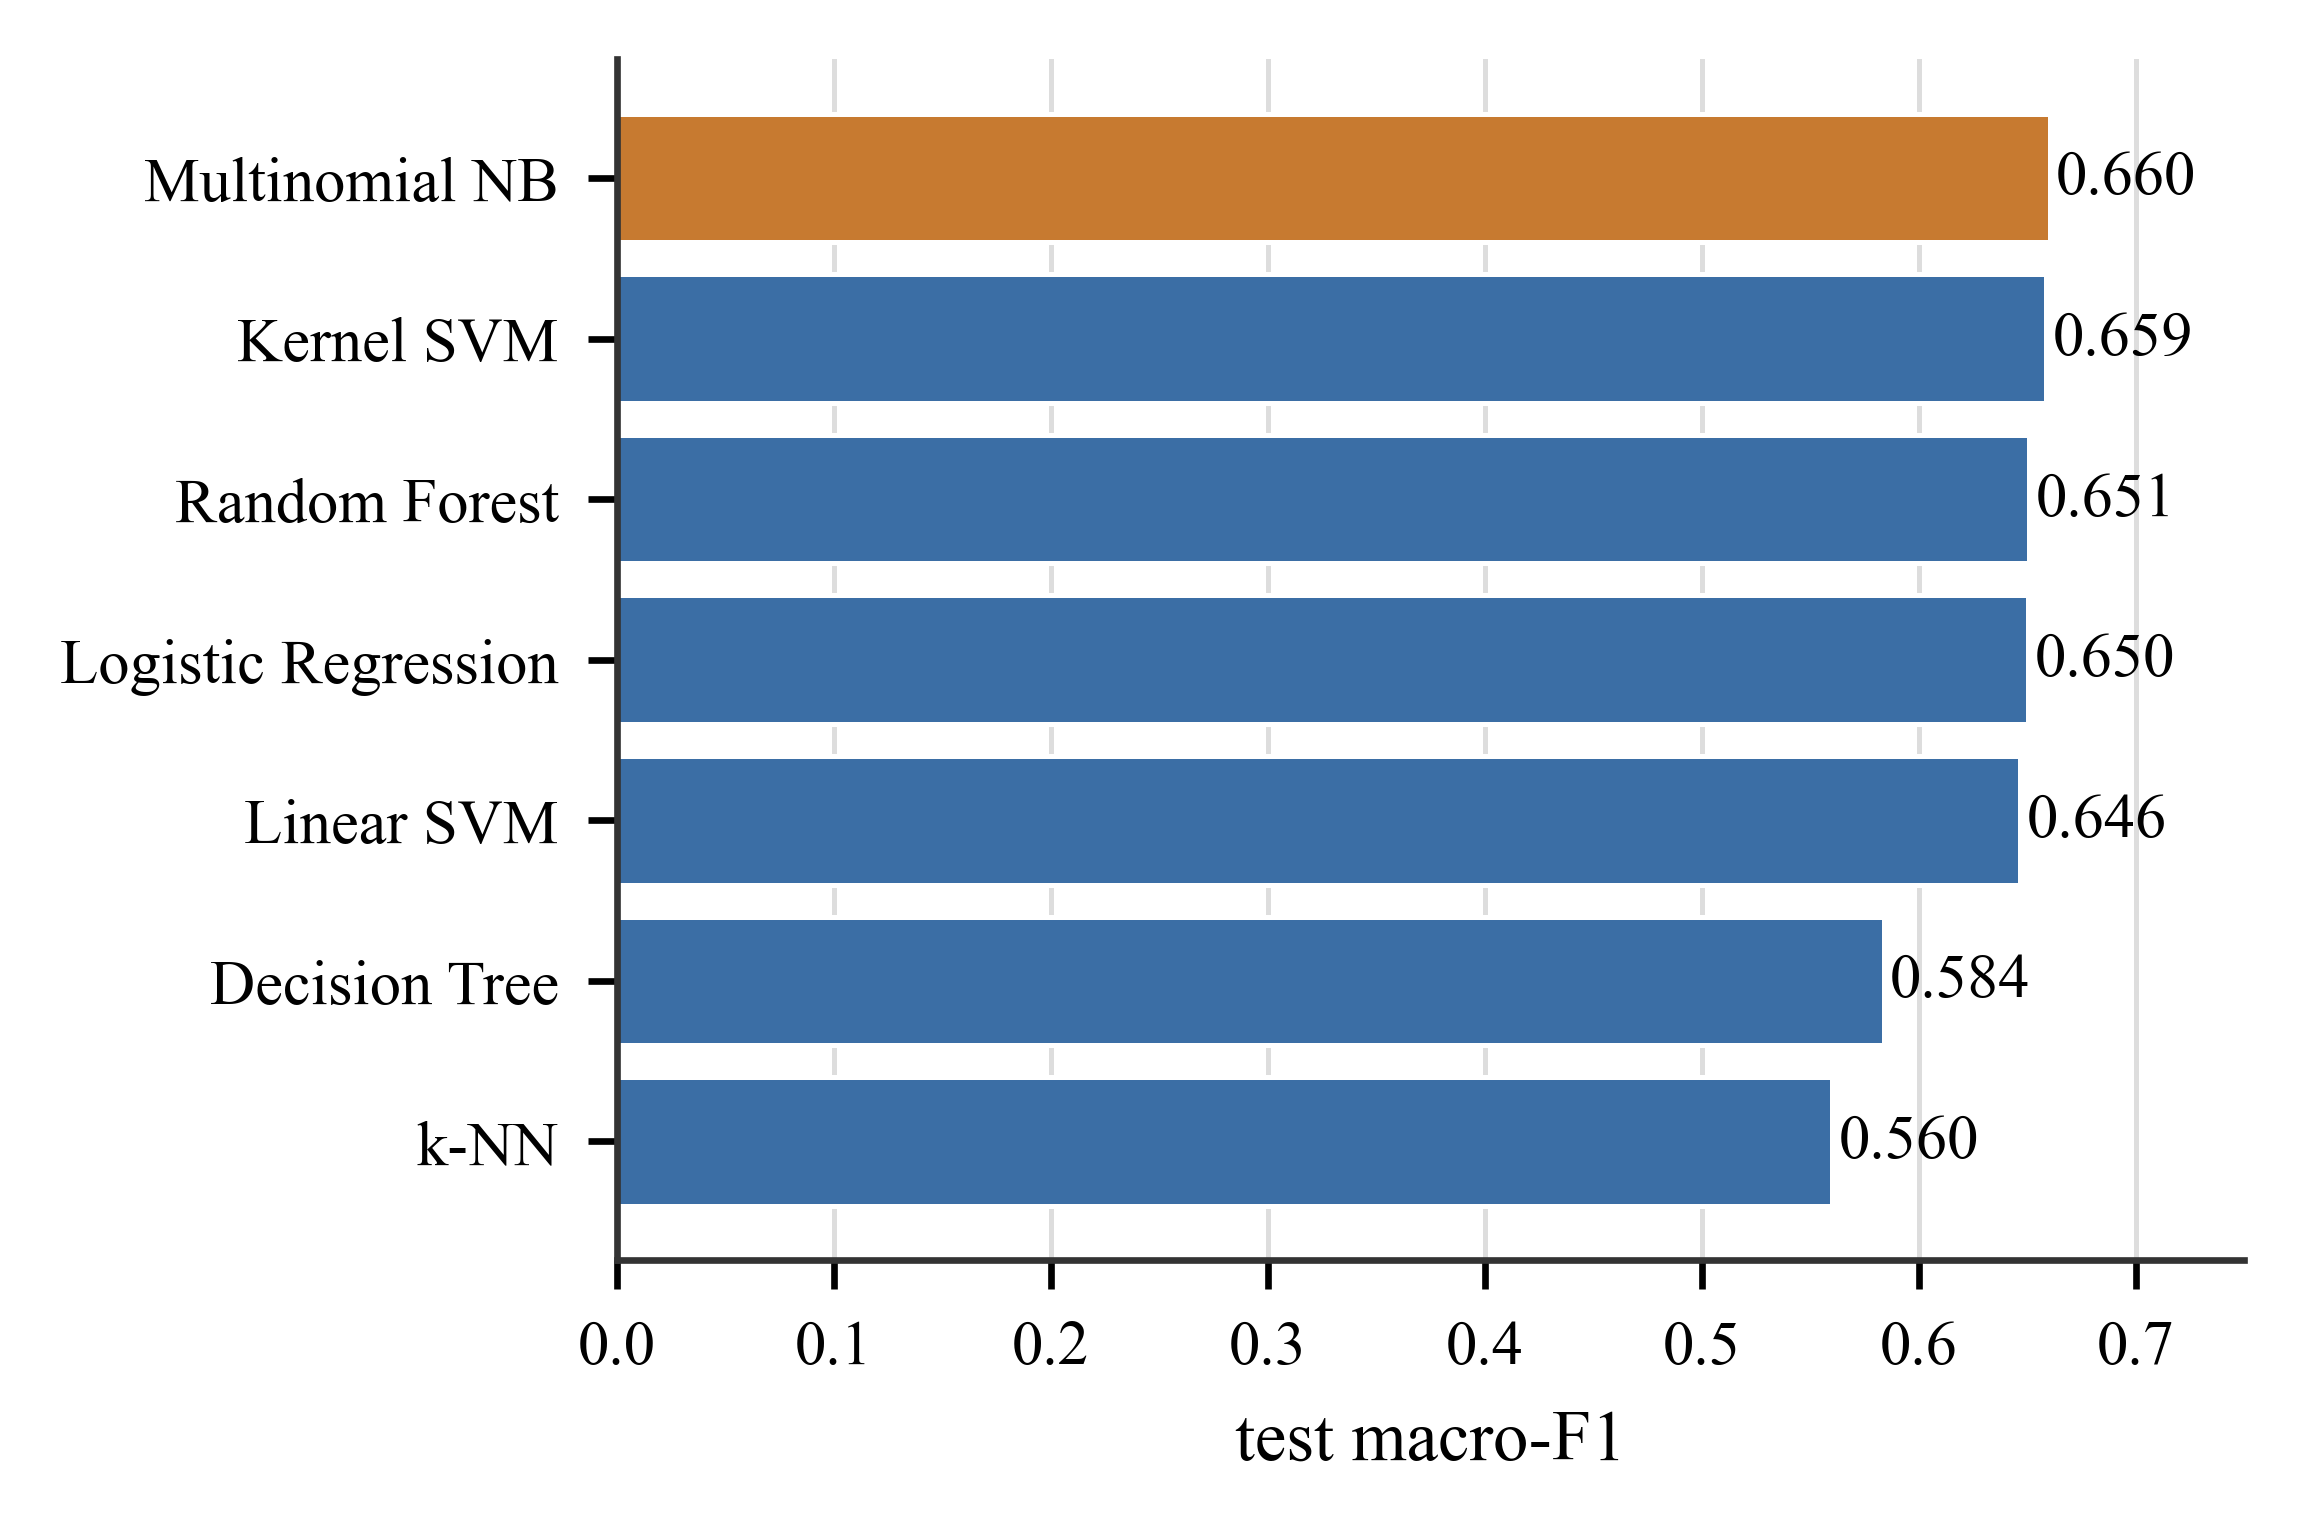
\includegraphics[width=0.92\columnwidth]{F_classical_ml.png}
\caption{Reproduced classical machine learning on \dset{Ben-Sarc} binary. Multinomial naive Bayes with trigram TF-IDF leads the family at 0.6602 macro-F1, with kernel SVM a thousandth behind.}
\label{fig:classical-ml}
\end{figure}

\subsection{Hardware, Software, and Hyperparameters}
\label{sec:hardware-and-hparams}

The authoritative 90-cell repeated experiment ran on one NVIDIA GeForce RTX 4090 (24\,GB), using CUDA 12.8, PyTorch 2.8.0, Transformers 4.57.6, pandas 3.0.3, and SciPy 1.18.0; its measured wall time was 3{,}484\,s (58.1\,min). Earlier reproduction, backbone, adversarial, ensemble, and enhanced-head notebooks used an NVIDIA A40 (48\,GB), PyTorch 2.1, Transformers 4.36, and scikit-learn 1.3 \cite{paszke2019pytorch,wolf2020transformers,pedregosa2011scikit}. Seeds are set in PyTorch, NumPy, and Python. Reporting both environments prevents the supporting single-run artifacts from being mistaken for reruns under the final environment. \Cref{tab:hparams} lists the shared transformer training settings.

\begin{table}[!t]
\centering
\caption{Transformer training settings. Primary denotes the repeated vanilla/FGM matrix; ``enhanced only'' denotes the earlier single dual-pooling run.}
\label{tab:hparams}
\footnotesize
\setlength{\tabcolsep}{2pt}
\begin{tabularx}{\columnwidth}{@{}lcX@{}}
\toprule
\textbf{Hyperparameter} & \textbf{Value} & \textbf{Notes} \\
\midrule
Optimizer & AdamW \cite{loshchilov2019adamw} & $\beta_1\!=\!0.9$, $\beta_2\!=\!0.999$, $\epsilon\!=\!10^{-8}$ \\
Base learning rate & $2\times 10^{-5}$ & primary warmup ratio $0.10$ \\
Head learning rate & $1\times 10^{-4}$ & enhanced only \\
Layer-wise decay $\xi$ & $0.95$ & enhanced only \\
Weight decay & $0.01$ & --- \\
Batch size & $32$ & no gradient accumulation \\
Max sequence length & $128$ / $192$ & primary / enhanced \\
Epochs & up to $8$ & early stopping, patience $2$ \\
Selection metric & validation only & criterion recorded per notebook; never test \\
Head dropout & $0.3$ & enhanced only \\
Label smoothing $s$ & $0.05$ & enhanced only (\cref{eq:label-smoothing}) \\
Evaluation batch size & $64$ & primary repeated matrix \\
FGM $\epsilon$ & $0.5$ & primary and ablations \\
AWP $\alpha$ (start) & $0.01$ (epoch $1$) & enhanced and ablation \\
\bottomrule
\end{tabularx}
\end{table}

\begin{table*}[!t]
\centering
\caption{Evidence hierarchy used to prevent incompatible artifacts from being combined. ``Primary'' results determine the abstract and conclusion; supporting tracks answer narrower questions.}
\label{tab:evidence-hierarchy}
\footnotesize
\setlength{\tabcolsep}{4pt}
\begin{tabularx}{\textwidth}{@{}lclX@{}}
\toprule
\textbf{Track} & \textbf{Scale} & \textbf{Role} & \textbf{Permitted interpretation} \\
\midrule
Vanilla/FGM repeated matrix & 90 cells & Primary & Five-seed means, transfer gaps, and matched effect sizes \\
Dataset-defined fixed targets & 60 paired contrasts & Primary sensitivity & Seed-wise target-relative loss and retention for both systems \\
Repeated calibration & 90 prediction files & Primary diagnostic & Source-validation temperature scaling; diagonal versus shifted ECE/Brier \\
Backbone benchmark & 5 backbones $\times$ 4 tasks & Supporting &
Native sequence-classification heads under a standardized training budget \\
Adversarial/epsilon ablation & 5 schemes + 4 budgets & Supporting & Single-run local sensitivity; no general adversarial-training claim \\
Reproduction/head/ensemble & Saved paired predictions & Supporting & Same-split item bootstrap or McNemar, limited to named checkpoints \\
\bottomrule
\end{tabularx}
\end{table*}

\subsection{Machine-Readable Result Provenance}
\label{sec:result-provenance}

The finalization notebook does not infer headline numbers from plot pixels or manually transcribed tables. It writes one row per system--source--seed--target run, derives summaries from that long-form record, and exports the statistical tests and audits as separate machine-readable files. The sanitized public per-example CSV files preserve target label,predicted label, and provenance fields. The manifest inventories finalized artifacts, while the run configuration records the model identifier, seeds, optimization settings, software versions, overlap policy, and wall time. This separation allows a reviewer to trace each primary claim to its generating record and prevents older single-run artifacts from silently overriding the repeated matrix. \Cref{tab:provenance-map} gives the claim-to-artifact map used during manuscript consistency checking.

\begin{table*}[!t]
\centering
\caption{Provenance map for primary claims. Paths are relative to the root of the public code repository. Prediction and split-manifest files contain hashes and numerical evidence but no comment text.}
\label{tab:provenance-map}
\scriptsize
\setlength{\tabcolsep}{3pt}
\begin{tabularx}{\textwidth}{@{}lXl@{}}
\toprule
\textbf{Claim or audit} & \textbf{Authoritative machine-readable artifact} & \textbf{Unit of record} \\
\midrule
All 90 evaluations &
\path{04_outputs/finalized_outputs/tables/18_transformer_cross_corpus_multiseed_runs.csv} &
system--source--seed--target \\

Means, standard deviations, and seed CIs &
\path{04_outputs/finalized_outputs/tables/18_transformer_cross_corpus_multiseed_summary.csv} &
system--source--target \\

FGM--vanilla resolution audit &
\path{04_outputs/finalized_outputs/tables/18_fgm_vs_vanilla_paired_seed_tests.csv} &
source--target paired contrast \\

Fixed-target uncertainty &
\path{04_outputs/finalized_outputs/tables/18_fixed_target_seedwise_sensitivity.csv} and
\path{04_outputs/finalized_outputs/tables/18_fixed_target_summary.csv} &
system--source--seed--target \\

Splits and exact-match controls &
\path{01_data/interim/split_manifests/*_hashed.csv} and
\path{04_outputs/finalized_outputs/tables/18_fixed_target_definition_audit.json} &
hashed item / target \\

Shift diagnostics &
\path{04_outputs/finalized_outputs/tables/18_cross_corpus_shift_audit.csv} and
\path{04_outputs/finalized_outputs/tables/18_shift_transfer_association.json} &
directed corpus pair \\

Configuration and inventory &
\path{04_outputs/finalized_outputs/tables/18_run_config.json} and
\path{04_outputs/finalized_outputs/MANIFEST_sha.json} &
complete run / artifact \\
\bottomrule
\end{tabularx}
\end{table*}

\subsection{Evaluation Metrics}
\label{sec:metrics}

The primary metric is macro-F1. For class $c$, with $\mathrm{TP}_c$, $\mathrm{FP}_c$, and $\mathrm{FN}_c$ the usual counts, precision is $\mathrm{Prec}(c)=\mathrm{TP}_c/(\mathrm{TP}_c+\mathrm{FP}_c)$, recall is $\mathrm{Rec}(c)=\mathrm{TP}_c/(\mathrm{TP}_c+\mathrm{FN}_c)$, and
\begin{equation}
\mathrm{F1}(c) = \frac{2\,\mathrm{Prec}(c)\,\mathrm{Rec}(c)}{\mathrm{Prec}(c)+\mathrm{Rec}(c)},
\label{eq:f1}
\end{equation}
\begin{equation}
\mathrm{macro\text{-}F1}=\frac{1}{C}\sum_{c=1}^{C}\mathrm{F1}(c),
\label{eq:macrof1}
\end{equation}
which gives every class equal weight regardless of frequency and so cannot be inflated by a majority-class-heavy predictor on \dset{BanglaSarc}. Accuracy is reported alongside for continuity with the reference paper.

Calibration asks a different question: not whether the arg-max is right, but whether the probability attached to it means anything. A model is perfectly calibrated when
\begin{equation}
\mathbb{P}\!\left(\hat{y}=y \;\middle|\; \max_c \hat{p}_c = q\right) = q \qquad \text{for all } q\in[0,1].
\label{eq:calibration-def}
\end{equation}
The ECE \cite{guo2017calibration,naeini2015ece} estimates the deviation from \cref{eq:calibration-def} by partitioning predictions into $M$ equal-width confidence bins $B_1,\ldots,B_M$ and averaging the gap,
\begin{equation}
\mathrm{ECE} = \sum_{m=1}^{M}\frac{|B_m|}{N}\,\bigl|\mathrm{acc}(B_m) - \mathrm{conf}(B_m)\bigr|,
\label{eq:ece}
\end{equation}
Here, \(N=\sum_{m=1}^{M}|B_m|\) is the number of evaluated examples.
with $\mathrm{acc}(B_m) = \tfrac{1}{|B_m|}\sum_{i\in B_m}\mathbb{1}[\hat{y}_i=y_i]$ and $\mathrm{conf}(B_m) = \tfrac{1}{|B_m|}\sum_{i\in B_m}\max_c\hat{p}_{i,c}$; we use $M\!=\!15$. The Brier score \cite{brier1950verification} is the mean squared error between predicted probabilities and one-hot labels,
\begin{equation}
\mathrm{Brier} = \frac{1}{N}\sum_{i=1}^{N}\sum_{c=1}^{C}\bigl(\hat{p}_{i,c}-y_{i,c}\bigr)^{2},
\label{eq:brier}
\end{equation}
and unlike ECE it is a proper scoring rule, so it penalizes miscalibration and inaccuracy together rather than binning them apart. Where a model is miscalibrated we fit a single temperature $T$ on validation logits,
\begin{equation}
\hat{p}^{\,T}_{i,c} = \frac{\exp(z_{i,c}/T)}{\sum_{c'}\exp(z_{i,c'}/T)},
\label{eq:tempsoftmax}
\end{equation}
\begin{equation}
T^{\star} = \arg\min_{T>0}\; -\!\!\sum_{i\in\mathcal{D}_{\mathrm{va}}}\!\log \hat{p}^{\,T}_{i,y_i},
\label{eq:temperature}
\end{equation}
noting that $\arg\max_c \hat{p}^{\,T}_{i,c} = \arg\max_c z_{i,c}$ for every $T>0$, so \cref{eq:temperature} cannot change a single prediction and leaves accuracy and macro-F1 exactly where they were.

\subsection{Statistical Testing}
\label{sec:stat-tests}

The inferential procedure follows the evidence hierarchy of \cref{tab:evidence-hierarchy}. Repeated source--target results are primary; saved item-level comparisons from earlier notebooks are supporting analyses. All inference is conditional on the one frozen 80/10/10 split: varying optimization seeds does not quantify uncertainty from redrawing train, validation, and test items.

For a fixed system and source--target cell, let $T_s$ be macro-F1 for seed $s$ and $S=5$. We report
\begin{equation}
\bar T\ \pm\ t_{0.975,S-1}\frac{s_T}{\sqrt S},
\qquad
s_T^2=\frac{1}{S-1}\sum_s(T_s-\bar T)^2,
\label{eq:seed-ci}
\end{equation}
which quantifies training-seed variation for that complete evaluation cell. To compare FGM with vanilla, the seed is matched and $d_s=T^{\mathrm{FGM}}_s-T^{\mathrm{vanilla}}_s$. An exact two-sided sign-flip test enumerates the $2^5$ vectors $(\eta_1d_1,\ldots,\eta_5d_5)$ for $\eta_s\in\{-1,+1\}$ and compares $|\bar d|$ with the resulting null distribution. With five nonzero matched differences, its smallest attainable two-sided raw $p$-value is $2/2^5=0.0625$. Consequently, this design cannot reject at 0.05 even before Holm adjustment, and the first Holm threshold for nine hypotheses is $0.05/9=0.0056$. The adjusted results are reported for transparency but cannot establish equivalence or absence of an effect; they show that this five-seed experiment is unable to resolve a systematic FGM advantage. Student-$t$ intervals are parametric descriptive summaries over five seeds, so an interval excluding zero (as on the BanglaSarc diagonal) and a nonsignificant exact test reflect different assumptions rather than a contradiction. This test targets a system effect across matched training seeds; it is distinct from a test that resamples test items while holding one trained model fixed.

For fixed-target loss, the target-trained and transferred scores are evaluated
on the same items and differenced within each system and seed. Reusing a seed
provides an experimental block: the paired value compares the same numbered
replicate under the same software, data-ordering convention, and evaluation
population. The source-trained and target-trained networks are nevertheless
optimized separately, so this blocking convention does not assert a natural
dependence between the fitted models. The twelve resulting Student-$t$
intervals---six directed pairs for each of two systems---are unadjusted,
parametric, fixed-split descriptive intervals. They do not provide simultaneous
95\% coverage and are not treated as twelve confirmatory hypothesis tests.
For older one-run artifacts, we retain prediction-level uncertainty. Percentile intervals use $B=2{,}000$ test-item bootstrap resamples \cite{efron1979bootstrap}. Direct macro-F1 contrasts use $B=5{,}000$ \emph{paired} resamples of the shared indices, reporting the percentile interval of the difference and twice the smaller tail mass about zero. McNemar's test \cite{mcnemar1947note} separately evaluates paired correctness from discordant counts $b$ (only model A correct) and $c$ (only model B correct),
\begin{equation}
\chi^{2}=\frac{(|b-c|-1)^2}{b+c}\ \dot{\sim}\ \chi^2_1.
\label{eq:mcnemar}
\end{equation}
McNemar therefore tests accuracy rather than macro-F1 and is labelled accordingly. The available frozen-encoder contrast is planned; other pairwise tests are secondary raw comparisons, not a multiplicity-adjusted ranking. The ensemble has only McNemar output, so no significance claim is made about its macro-F1 difference.

One more quantity does much of the work in \cref{sec:results}. Repeating a configuration over seeds $\mathcal{S}$ and recording test macro-F1 $T_s$ gives the seed standard deviation
\begin{equation}
\sigma_{\mathrm{seed}} = \sqrt{\frac{1}{|\mathcal{S}|-1}\sum_{s\in\mathcal{S}}\bigl(T_s - \bar{T}\bigr)^2},
\label{eq:seed-std}
\end{equation}
a descriptive scale for movement when only the optimization seed changes. It is not a decision rule: the paired analyses above, not comparison with $\sigma_{\mathrm{seed}}$, determine what the experiment can resolve.

\section{Results and Analysis}
\label{sec:results}

The results first compare frozen and fully fine-tuned encoders, then report paired comparisons, adversarial ablations, and five-seed stability. The repeated cross-corpus matrix and fixed-target sensitivity are the primary evidence; the exploratory head, ensemble, calibration, and error analyses are labelled according to their actual replication level.

\subsection{Full Fine-Tuning Is the Real Gain}
\label{sec:bangla-baseline}

Before the final repeated experiment, a saved vanilla BanglaBERT run reached 0.8025 macro-F1 at 80.30\% accuracy on Ben-Sarc ($n_{\mathrm{te}}=2{,}563$). This is a separate supporting run from the multi-backbone BanglaBERT cell (0.7981) and the final five-seed vanilla mean (0.7914); these values are neither averaged nor selected post hoc. In the authoritative FGM series, the three in-domain means are 0.7984 on Ben-Sarc, 0.9817 on BanglaSarc, and 0.7595 on BanglaSarc3 binary. Across these variants, the stable high-level conclusion is that end-to-end adaptation materially exceeds the available frozen-encoder reproduction.


\subsection{Multi-Backbone Comparison}
\label{sec:multibackbone-results}

\Cref{tab:multibackbone} compares the five encoders across the four task variants under a standardized training budget, and \cref{fig:multibackbone} shows the three binary tasks as a heat map. BanglaBERT takes the best mean macro-F1, narrowly ahead of MuRIL, and the two Bengali-or-Indic models clear the general multilinguals comfortably.

The margin is not uniform. BanglaBERT and MuRIL differ by only 0.001 on Ben-Sarc, and MuRIL is higher on BanglaSarc3 binary. BanglaBERT has the highest four-task mean while using fewer parameters than MuRIL. Because each cell is a single run, close rows are descriptive rather than a definitive encoder ranking.

\begin{table*}[!t]
\centering
\caption{Multi-backbone macro-F1 across the four task variants. Vanilla full fine-tuning, single run, normalized-exact-match-controlled splits. BS = \dset{BanglaSarc}, BS3 = \dset{BanglaSarc3}.}
\label{tab:multibackbone}
\small
\setlength{\tabcolsep}{4pt}
\begin{tabular}{@{}lccccc@{}}
\toprule
\textbf{Backbone} & {\bfseries \dset{Ben-Sarc}} & \textbf{BS bin.} & \textbf{BS3 bin.} & \textbf{BS3 tern.} & \textbf{Mean} \\
\midrule
BanglaBERT & \textbf{0.7981} & \textbf{0.9742} & 0.7365 & \textbf{0.6351} & \textbf{0.7860} \\
MuRIL & 0.7971 & 0.9672 & \textbf{0.7468} & 0.6187 & 0.7825 \\
XLM-RoBERTa & 0.7807 & 0.9328 & 0.7291 & 0.6378 & 0.7701 \\
Sagorsarker BB & 0.7510 & 0.9437 & 0.7358 & 0.5942 & 0.7562 \\
mBERT & 0.7428 & 0.9420 & 0.7286 & 0.5910 & 0.7511 \\
\bottomrule
\end{tabular}
\end{table*}

\begin{figure}[tb]
\centering
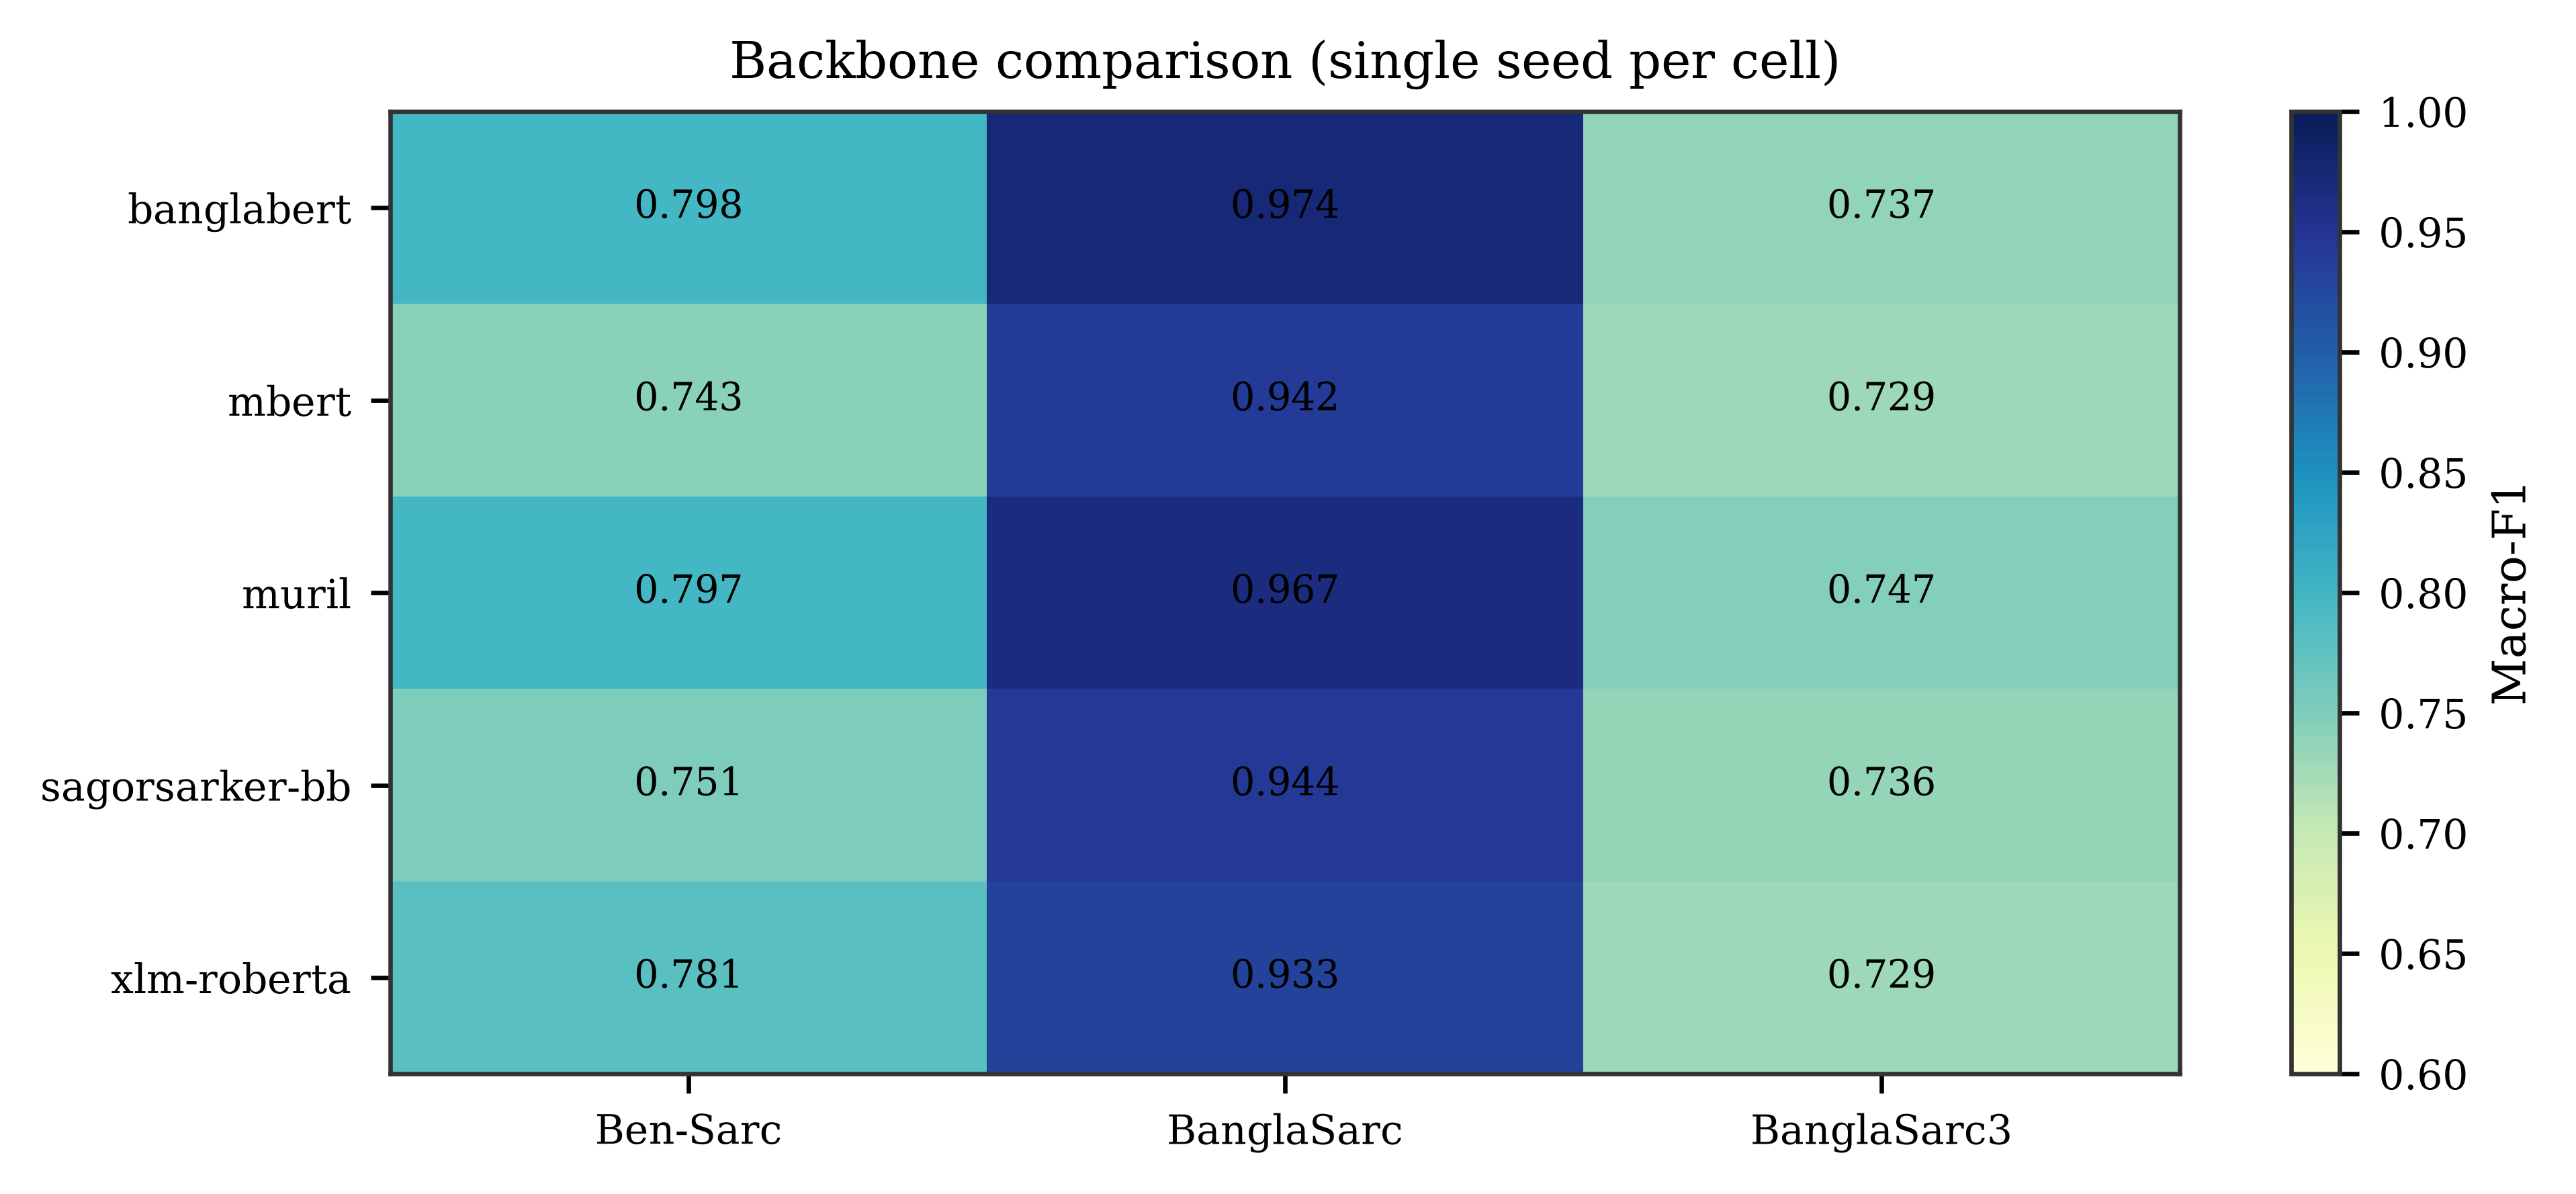
\includegraphics[width=0.99\columnwidth]{F_multibackbone.png}
\caption{Single-run macro-F1 of the five encoders on the three binary tasks under a standardized training budget. BanglaBERT and MuRIL lead on Ben-Sarc and BanglaSarc; because each cell is one run, near-tied rows are read as descriptive rather than as a fixed ranking (cf. \cref{tab:multibackbone}).}
\label{fig:multibackbone}
\end{figure}

\subsection{What Separates From Full Fine-Tuning, and What Does Not}
\label{sec:significance-results}

\Cref{tab:bootstrap-mcnemar} gives paired comparisons between the exploratory enhanced run and available Ben-Sarc prediction files. It separates the large frozen-to-fine-tuned gap from the negligible enhanced-to-vanilla difference, but it is not the repeated-seed estimate.

The first half is the clear result. The exploratory enhanced configuration exceeds every reproduced reference baseline. Against the strongest available frozen Bengali-BERT substitute, the macro-F1 gap is 0.0594 with a paired-bootstrap 95\% interval of $[0.0432,\,0.0764]$ that excludes zero, and McNemar gives $\chi^2\!=\!50.34$ at $p\!=\!1.3\times10^{-12}$. This comparison is valid for the evaluated substitute checkpoint; it does not reconstruct predictions from the withdrawn checkpoint.

The second half limits the modeling claim. Against vanilla full fine-tuning, the exploratory run differs by only 0.0013 macro-F1, with a paired-bootstrap interval of $[-0.0092,\,0.0125]$ and $p=0.7912$; McNemar similarly gives $p=0.8843$. XLM-RoBERTa is lower by 0.0231 macro-F1 (95\% CI $[0.0087,0.0379]$, raw paired-bootstrap $p=0.0008$). For the stacking ensemble, McNemar gives $p=0.1093$ for paired correctness; no paired-bootstrap macro-F1 test was saved, so we do not label its macro-F1 difference significant or nonsignificant.

Full fine-tuning over the evaluated frozen baselines is a large difference on both paired tests; differences within the stronger transformer group are smaller and require experiment-specific interpretation. This motivates reporting uncertainty rather than inferring a general method effect from a single score.

\begin{table*}[!t]
\centering
\caption{Paired tests on \dset{Ben-Sarc} binary, using the exploratory enhanced run (0.8038) as the index model. McNemar tests paired correctness; $\Delta$F1 and $p_{\mathrm{PB}}$ are from a 5{,}000-resample paired bootstrap of macro-F1. Values are raw; secondary comparisons are not a multiplicity-adjusted ranking.}
\label{tab:bootstrap-mcnemar}
\small
\setlength{\tabcolsep}{3.5pt}
\begin{tabular}{@{}lcccc@{}}
\toprule
\textbf{Comparator} & \textbf{macro-F1} & \textbf{McNemar p} & \textbf{F1 difference [95\% CI]} & \textbf{Bootstrap p} \\
\midrule
Frozen mBERT (ref.) & 0.6916 & $1.7\!\times\!10^{-28}$ & 0.1122 [0.0930, 0.1315] & $<0.0004$ \\
Frozen Sagorsarker (ref.) & 0.6921 & $<10^{-15}$ & 0.1117 [0.0922, 0.1320] & $<0.0004$ \\
Frozen Bengali-BERT substitute & 0.7444 & $1.3\!\times\!10^{-12}$ & 0.0594 [0.0432, 0.0764] & $<0.0004$ \\
mBERT backbone & 0.7428 & $6.6\!\times\!10^{-13}$ & 0.0611 [0.0448, 0.0779] & $<0.0004$ \\
Sagorsarker backbone & 0.7510 & $2.8\!\times\!10^{-9}$ & 0.0528 [0.0361, 0.0705] & $<0.0004$ \\
XLM-RoBERTa backbone & 0.7807 & $2.5\!\times\!10^{-3}$ & 0.0231 [0.0087, 0.0379] & 0.0008 \\
Vanilla BanglaBERT & 0.8025 & 0.8843 & 0.0013 [$-0.0092$, 0.0125] & 0.7912 \\
\bottomrule
\end{tabular}
\end{table*}


\subsection{Adversarial Training Ablation}
\label{sec:adversarial-results}

Under the matched native-head, seed-42 protocol, every adversarial score is at or below vanilla full fine-tuning (\cref{tab:adv-schemes}). Paired bootstrap against vanilla gives $\Delta=-0.0034$ for FGM (95\% CI $[-0.0133,0.0065]$, $p=0.5208$) and $\Delta=-0.0041$ for FreeLB (95\% CI $[-0.0159,0.0081]$, $p=0.5012$). AWP is lower by 0.0123 (95\% CI $[-0.0233,-0.0011]$, $p=0.0328$). The saved matched FGM+AWP run reaches 0.7994 but has no separate paired-bootstrap row in the finalization notebook; we therefore report its effect size without attaching a significance label.

The enhanced dual-pooling run is a different experiment. It reaches 0.8038 and differs from vanilla by 0.0013 (95\% CI $[-0.0092,0.0125]$, $p=0.7912$), but it changes several components simultaneously and cannot be used to infer an FGM, AWP, head, or label-smoothing effect. The $\epsilon$ sweep peaks on validation macro-F1 at 0.5, while test macro-F1 varies non-monotonically (\cref{fig:eps-sweep}). These results do not reproduce a benefit from adversarial training under the evaluated implementations.

\begin{table}[!t]
\centering
\caption{Adversarial-scheme ablation on \dset{Ben-Sarc} binary under a matched native-head protocol. No scheme exceeds the vanilla full-fine-tuning baseline.}
\label{tab:adv-schemes}
\footnotesize
\setlength{\tabcolsep}{2pt}
\begin{tabular}{@{}lcc@{}}
\toprule
\textbf{Scheme} & \textbf{Test macro-F1} & \textbf{Difference vs.\ vanilla} \\
\midrule
Vanilla full fine-tuning & \textbf{0.8025} & --- \\
FGM + AWP & 0.7994 & $-0.0031$ \\
FGM ($\epsilon\!=\!0.5$) & 0.7991 & $-0.0034$ \\
FreeLB ($k\!=\!3$) & 0.7984 & $-0.0041$ \\
AWP only & 0.7902 & $-0.0123$ \\
\bottomrule
\end{tabular}
\end{table}

\begin{figure}[!t]
\centering
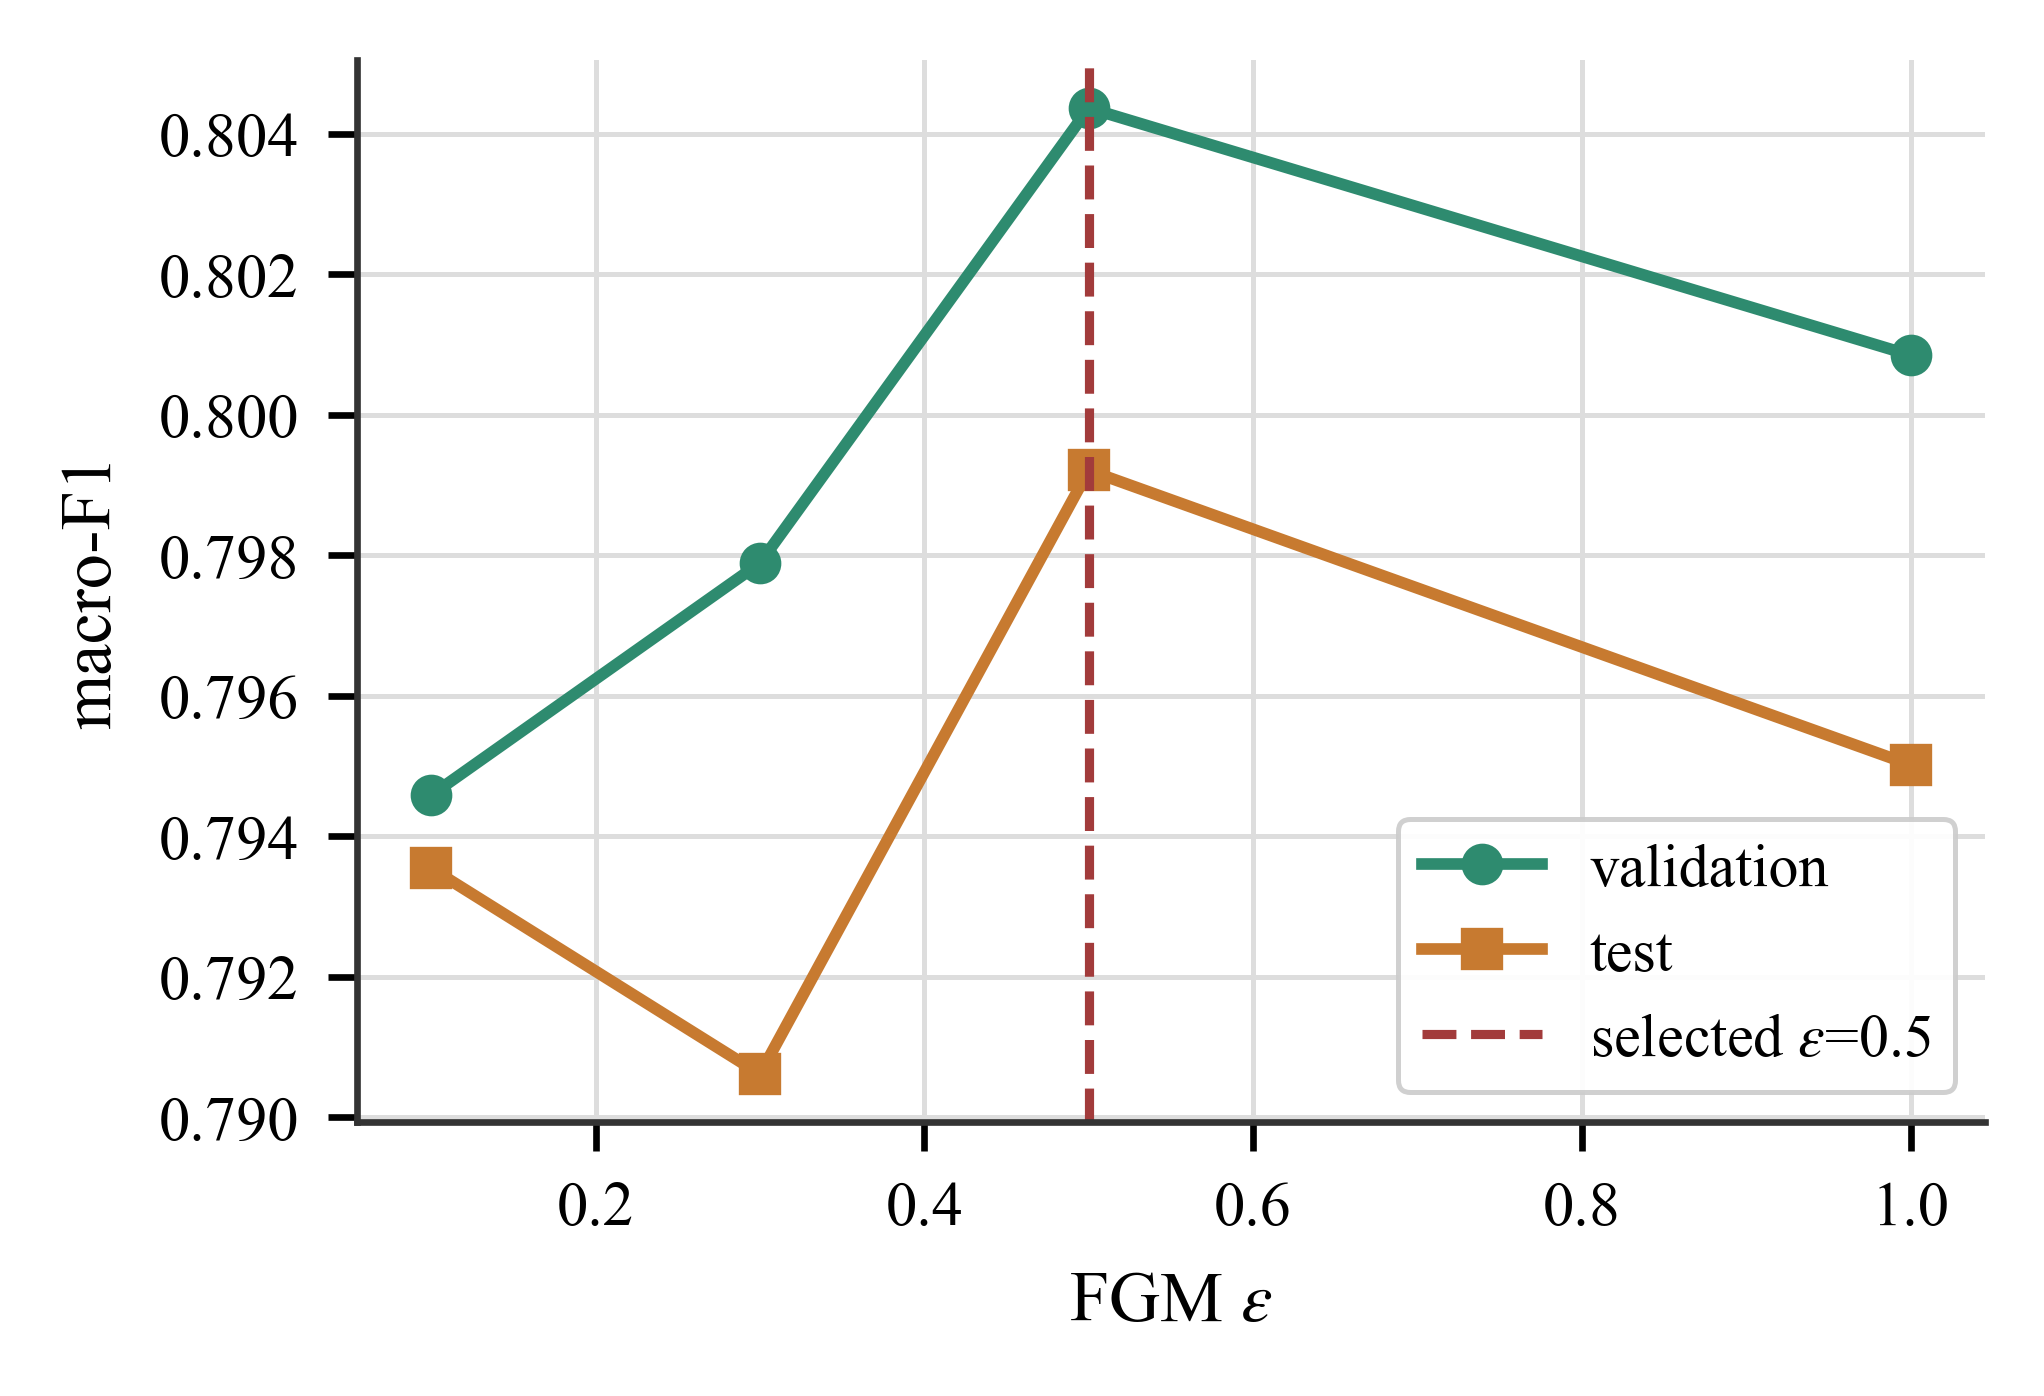
\includegraphics[width=0.92\columnwidth]{F_epsilon_sweep.png}
\caption{Single-seed FGM perturbation-budget sweep on \dset{Ben-Sarc} binary. Validation macro-F1 is highest at $\epsilon=0.5$; the corresponding test macro-F1 values are 0.7935, 0.7906, 0.7992, and 0.7950 for $\epsilon=0.1,0.3,0.5,1.0$.}
\label{fig:eps-sweep}
\end{figure}

All checkpoint choices follow the validation criterion recorded in the relevant notebook; no test-set result is used for selection.

\subsection{Seed Stability: Measuring the Noise Floor}
\label{sec:multiseed-results}

The final experiment repeats \emph{both} native-head BanglaBERT systems over seeds 42, 1, 7, 123, and 2024 for every matrix cell. \Cref{tab:multiseed} isolates the Ben-Sarc diagonal. FGM averages $0.7984\pm0.0035$ macro-F1 and vanilla averages $0.7914\pm0.0085$; their matched mean difference is 0.0070, but its 95\% seed-level interval $[-0.0008,0.0148]$ includes zero. The strongest FGM seed is 1 at 0.8033. \Cref{fig:seed-stability} plots the seed-wise in-domain macro-F1 for both systems on all three source corpora. The older 0.8038 enhanced result is a different, single-run architecture and is not a member of either repeated series.

The lower observed spread of FGM on this diagonal is descriptive: five seeds are insufficient to claim a general variance-reduction effect. We use the repeated means for headline performance and exact matched-seed tests for system comparisons, while keeping all single-run ablations secondary.

\begin{table}[!t]
\centering
\caption{Matched five-seed Ben-Sarc diagonal results for the native-head BanglaBERT systems. Scores are test macro-F1.}
\label{tab:multiseed}
\footnotesize
\setlength{\tabcolsep}{2pt}
\begin{tabular}{@{}lcc@{}}
\toprule
\textbf{Seed} & \textbf{Vanilla} & \textbf{FGM} \\
\midrule
42 & 0.7889 & 0.7993 \\
1 & 0.7997 & \textbf{0.8033} \\
7 & 0.7896 & 0.7947 \\
123 & 0.7995 & 0.7993 \\
2024 & 0.7794 & 0.7953 \\
\midrule
\textbf{Mean} & 0.7914 & \textbf{0.7984} \\
\textbf{Std.} & 0.0085 & \textbf{0.0035} \\
\bottomrule
\end{tabular}
\end{table}

\begin{figure*}[tp]
\centering
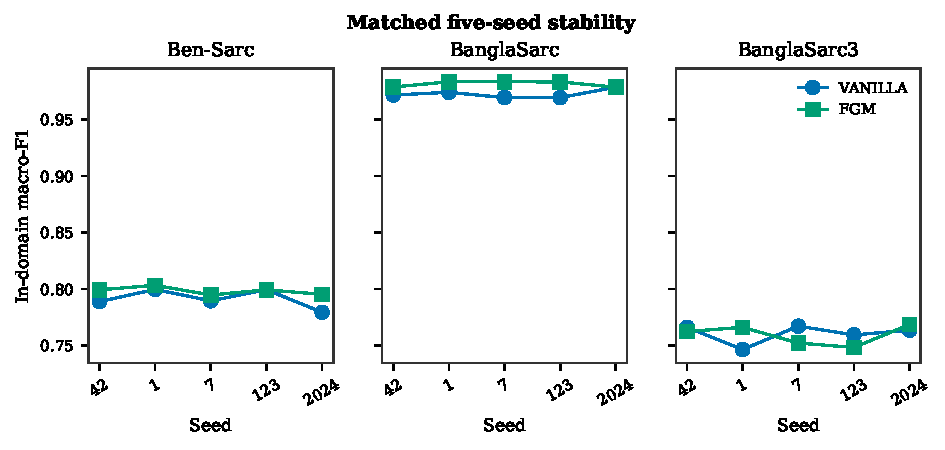
\includegraphics[width=0.80\textwidth]{F18_seed_stability}
\caption{Seed-wise in-domain macro-F1 for vanilla and FGM on all three source corpora. Lines connect matched seeds and visualize training variation. The vertical scale is expanded to make within-corpus movement visible; inference uses the numerical paired differences rather than visual separation.}
\label{fig:seed-stability}
\end{figure*}

\subsection{Cross-Corpus Transfer}
\label{sec:cross-dataset-results}

\Cref{tab:transfer} gives the repeated normalized-exact-match-controlled matrices of \cref{eq:repeated-transfer}, and \cref{fig:transfer-heatmaps} shows the two systems as heat maps. FGM averages 0.8465 on the three diagonal cells but only 0.5364 across the six directed off-diagonal cells; vanilla averages 0.8416 and 0.5379, respectively. \Cref{fig:indomain-transfer} contrasts the in-domain and cross-corpus distributions for both systems. FGM therefore changes neither the qualitative pattern nor the mean transfer level.

The Ben-Sarc FGM row is the best-behaved: 0.7984 in-domain, 0.5956 on BanglaSarc, and 0.6490 on BanglaSarc3, yielding $\Gamma=0.1761$. By contrast, BanglaSarc obtains 0.9817 in-domain but only 0.3460 and 0.3341 outside its corpus, so $\Gamma=0.6416$. BanglaSarc3 has the smallest gap, 0.1126. These off-diagonal values indicate severe degradation; we do not call them ``chance'' because macro-F1 chance behavior depends on class balance and the prediction rule.The exceptional BanglaSarc diagonal is conditional on this released corpus and
frozen split. Normalized exact matching cannot detect semantic or template-level
near-duplicates, so 0.9817 is not interpreted as deployment-level performance.

Two patterns generalize. \emph{(P1) In-domain rank does not predict transfer rank:} BanglaSarc is first in-domain and last by mean outgoing transfer. \emph{(P2) Transfer is asymmetric:} for example, FGM trained on BanglaSarc3 reaches 0.6700 on Ben-Sarc, whereas the reverse direction is 0.6490. The more extreme BanglaSarc-source rows reflect near-collapse of sarcastic-class recall, examined below.

An earlier TF--IDF cross-corpus output used train-only rather than all-source overlap filtering. Because it is not protocol-matched and is inexpensive but was not rerun, it is excluded from the comparative evidence and retained only in the project archive. The in-domain classical reproduction remains relevant to same-split historical comparison.

This qualifies how earlier cross-set results should be read. Lora et al.\ \cite{lora2023transformer} evaluate a Ben-Sarc-trained model on BanglaSarc and interpret the outcome as robustness. In our five-seed FGM matrix that direction is 0.5956 (95\% CI [0.5519, 0.6392]), whereas the reverse is 0.3460 ([0.3405, 0.3515]). One directional cell hides both uncertainty and strong asymmetry.

\begin{table*}[!t]
\centering
\caption{Five-seed normalized-exact-match-controlled cross-corpus macro-F1. Cells are mean [Student-$t$ 95\% CI]. Off-diagonal evaluation excludes normalized exact overlap with the complete source corpus. Retained target sizes are stated in the text.}
\label{tab:transfer}
\scriptsize
\setlength{\tabcolsep}{2.5pt}
\begin{tabular}{@{}llcccc@{}}
\toprule
\textbf{System} & \textbf{Source} & \textbf{Ben-Sarc} & \textbf{BanglaSarc} & \textbf{BanglaSarc3} & \textbf{Gap} \\
\midrule
FGM & Ben-Sarc & \textbf{0.7984} [0.7941, 0.8027] & 0.5956 [0.5519, 0.6392] & 0.6490 [0.6384, 0.6597] & 0.1761 \\
FGM & BanglaSarc & 0.3460 [0.3405, 0.3515] & \textbf{0.9817} [0.9785, 0.9848] & 0.3341 [0.3288, 0.3393] & 0.6416 \\
FGM & BanglaSarc3 & 0.6700 [0.6636, 0.6764] & 0.6238 [0.5662, 0.6814] & \textbf{0.7595} [0.7485, 0.7705] & 0.1126 \\
\midrule
Vanilla & Ben-Sarc & \textbf{0.7914} [0.7809, 0.8019] & 0.5906 [0.5511, 0.6302] & 0.6441 [0.6270, 0.6612] & 0.1740 \\
Vanilla & BanglaSarc & 0.3462 [0.3419, 0.3505] & \textbf{0.9728} [0.9680, 0.9776] & 0.3374 [0.3306, 0.3441] & 0.6310 \\
Vanilla & BanglaSarc3 & 0.6675 [0.6582, 0.6768] & 0.6415 [0.6011, 0.6818] & \textbf{0.7605} [0.7501, 0.7710] & 0.1060 \\
\bottomrule
\end{tabular}
\end{table*}

Off-diagonal filtering removes no items in four directed pairs; it removes 29 of 791 BanglaSarc3 test items when BanglaSarc is the source and 28 of 464 BanglaSarc test items when BanglaSarc3 is the source. The retained sizes are therefore 762 and 436 in those two cells, respectively, and the complete target test size elsewhere. Because this pair-specific policy changes the target population, scores across source rows should not be compared as though every row used identical items.

\Cref{tab:fixed-target} addresses that comparability issue using the
dataset-defined populations of \cref{eq:fixed-target}. Mean target-relative
retention remains only 0.433--0.851 for FGM and 0.438--0.844 for vanilla. Every
unadjusted descriptive paired-loss interval is above zero, including the
smallest FGM loss, Ben-Sarc$\rightarrow$BanglaSarc3, at 0.1138
[0.0955, 0.1322]. Variable target composition and BanglaSarc's unusually high
diagonal therefore do not account for the observed pattern on these fixed
populations. These quantities control target difficulty descriptively, but
corpus construction, label policy, and platform remain bundled.

\begin{table*}[!t]
\centering
\caption{Dataset-defined fixed-target sensitivity for both systems. Entries are
means [unadjusted Student-$t$ 95\% CI] of five seed-wise paired losses or
retentions from \cref{eq:target-relative}; all transferred and target-trained
scores use the same items and experimental seed block. Intervals are descriptive
and conditional on the frozen split.}
\label{tab:fixed-target}
\scriptsize
\setlength{\tabcolsep}{3pt}
\begin{tabular}{@{}lllrrr@{}}
\toprule
\textbf{System} & \textbf{Source} & \textbf{Target} & \textbf{Fixed n} & \textbf{Loss $L_{j\rightarrow k}$} & \textbf{Retention $R_{j\rightarrow k}$} \\
\midrule
FGM & Ben-Sarc & BanglaSarc & 436 & 0.3880 [0.3410, 0.4349] & 0.6045 [0.5568, 0.6523] \\
FGM & Ben-Sarc & BanglaSarc3 & 762 & 0.1138 [0.0955, 0.1322] & 0.8506 [0.8286, 0.8726] \\
FGM & BanglaSarc & Ben-Sarc & 2{,}563 & 0.4524 [0.4441, 0.4606] & 0.4334 [0.4253, 0.4415] \\
FGM & BanglaSarc & BanglaSarc3 & 762 & 0.4268 [0.4119, 0.4418] & 0.4391 [0.4277, 0.4505] \\
FGM & BanglaSarc3 & Ben-Sarc & 2{,}563 & 0.1284 [0.1207, 0.1362] & 0.8392 [0.8299, 0.8484] \\
FGM & BanglaSarc3 & BanglaSarc & 436 & 0.3572 [0.2995, 0.4148] & 0.6359 [0.5772, 0.6946] \\
\midrule
Vanilla & Ben-Sarc & BanglaSarc & 436 & 0.3838 [0.3385, 0.4291] & 0.6053 [0.5605, 0.6502] \\
Vanilla & Ben-Sarc & BanglaSarc3 & 762 & 0.1187 [0.1041, 0.1333] & 0.8440 [0.8250, 0.8630] \\
Vanilla & BanglaSarc & Ben-Sarc & 2{,}563 & 0.4452 [0.4315, 0.4590] & 0.4375 [0.4273, 0.4477] \\
Vanilla & BanglaSarc & BanglaSarc3 & 762 & 0.4236 [0.4155, 0.4318] & 0.4433 [0.4363, 0.4504] \\
Vanilla & BanglaSarc3 & Ben-Sarc & 2{,}563 & 0.1239 [0.1064, 0.1414] & 0.8436 [0.8234, 0.8638] \\
Vanilla & BanglaSarc3 & BanglaSarc & 436 & 0.3308 [0.2895, 0.3721] & 0.6598 [0.6176, 0.7020] \\
\bottomrule
\end{tabular}
\end{table*}

\begin{figure*}[!t]
\centering
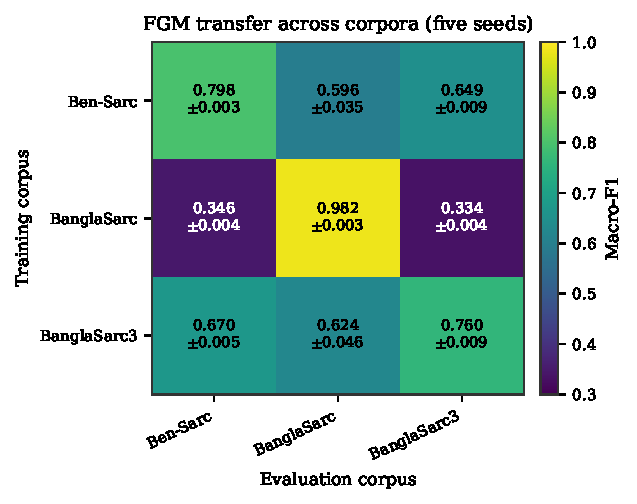
\includegraphics[width=0.48\textwidth]{F18_cross_dataset_fgm_multiseed}\hfill
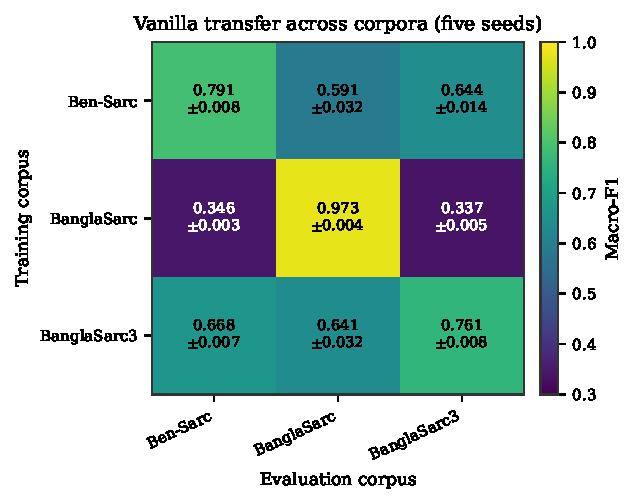
\includegraphics[width=0.48\textwidth]{F18_cross_dataset_vanilla_multiseed}
\caption{Five-seed mean cross-corpus macro-F1 for FGM (left) and vanilla (right). Both systems exhibit the same strong diagonal and asymmetric transfer failures.}
\label{fig:transfer-heatmaps}
\end{figure*}

\begin{figure}[!t]
\centering
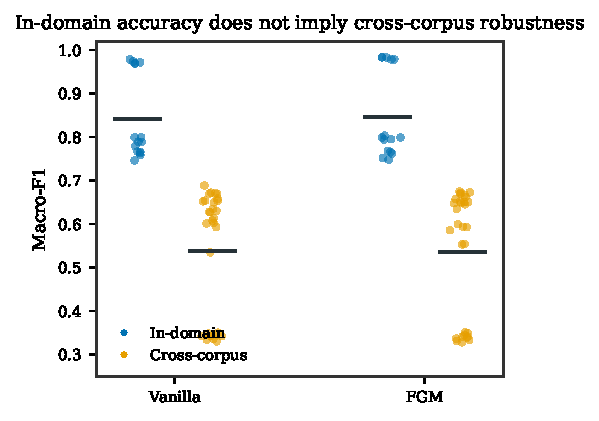
\includegraphics[width=0.92\columnwidth]{F18_indomain_vs_transfer_multiseed}
\caption{In-domain versus cross-corpus macro-F1 for vanilla and FGM, pooled over all directed source--target cells; horizontal bars mark the group means. For both systems the in-domain scores cluster far above the cross-corpus scores, so a strong in-domain result does not imply cross-corpus robustness.}
\label{fig:indomain-transfer}
\end{figure}

\subsection{Matched FGM--Vanilla Inference}
\label{sec:paired-seed-results}

The repeated design permits a direct system comparison that the older single-run ablation could not provide, but it is treated as an effect-size analysis rather than a confirmatory test. Across the nine cells, matched FGM-minus-vanilla means range from $-0.0177$ to 0.0089 (\cref{fig:fgm-vanilla-differences}). Every Student-$t$ interval except the BanglaSarc diagonal includes zero; that diagonal's interval [0.0016, 0.0161] excludes zero, whereas its assumption-light exact sign-flip value is $p=0.125$. As established in \cref{sec:stat-tests}, five seeds make a two-sided exact $p<0.05$ impossible. The complete nine-cell exact/Holm table remains in \path{04_outputs/finalized_outputs/tables/18_fgm_vs_vanilla_paired_seed_tests.csv} for audit, but it is not promoted as inferential evidence. The defensible conclusion is that small FGM effects remain unresolved while both systems exhibit the same large transfer degradation.

\begin{figure*}[!t]
\centering
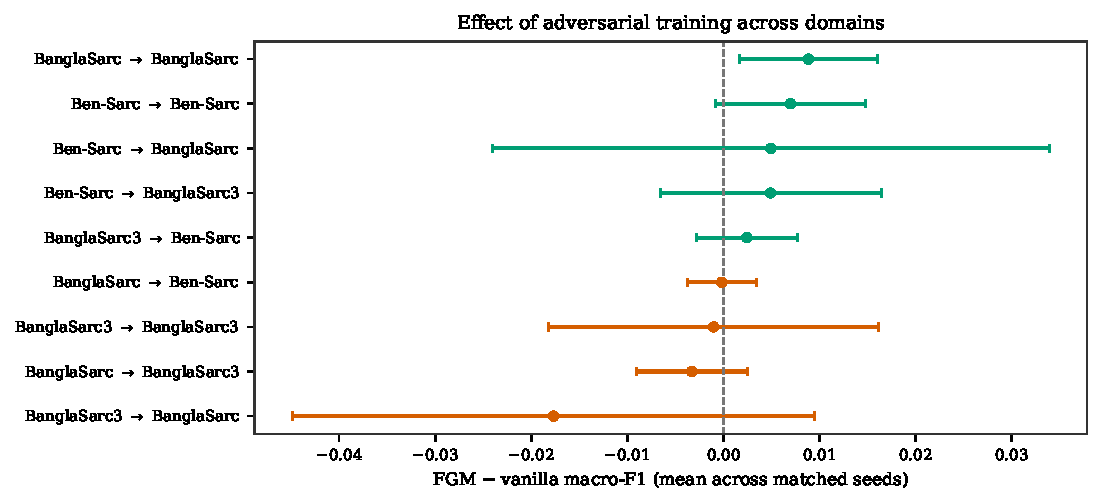
\includegraphics[width=0.82\textwidth]{F18_fgm_vs_vanilla_transfer}
\caption{FGM--vanilla differences over all repeated source--target cells. Error bars are 95\% confidence intervals over five matched seeds; the dashed line marks no difference.}
\label{fig:fgm-vanilla-differences}
\end{figure*}

\subsection{Shift Audit and Transfer Error Asymmetry}
\label{sec:shift-audit-results}

To move beyond a generic statement that the corpora differ, we audit token-vocabulary Jaccard similarity, target token out-of-vocabulary rate relative to the source training vocabulary, character TF--IDF centroid cosine similarity, and absolute positive-rate gap. Across the six off-diagonal cells, these span 0.054--0.256, 0.199--0.619, 0.780--0.921, and 0.0006--0.155, respectively (\cref{tab:shift-audit}). They document observable distribution differences but do not identify a causal mechanism.

An exploratory association between character TF--IDF centroid cosine similarity and five-seed mean FGM transfer macro-F1 gives Spearman $\rho=0.43$ with $p=0.40$ over only six directed cells (\cref{fig:shift-transfer}). The positive direction is compatible with greater lexical similarity accompanying better transfer, but the sample is far too small for inference or causal attribution. Class-wise recall reveals a more actionable failure: on BanglaSarc$\rightarrow$BanglaSarc3, class-0 recall is 0.987 whereas class-1 recall is 0.009. Macro-F1 exposes that near-collapse even though accuracy remains close to the majority-class rate.

\begin{table*}[!t]
\centering
\caption{Directed off-diagonal shift audit and five-seed FGM transfer. OOV is the target token rate outside the source-training vocabulary; cosine compares character TF--IDF centroids; label gap is the absolute positive-rate difference.}
\label{tab:shift-audit}
\scriptsize
\setlength{\tabcolsep}{3pt}
\begin{tabular}{@{}llrrrrrr@{}}
\toprule
\textbf{Source} & \textbf{Target} & \textbf{Token Jaccard} & \textbf{Target OOV} & \textbf{Centroid cosine} & \textbf{Label gap} & \textbf{Clean n} & \textbf{FGM F1} \\
\midrule
Ben-Sarc & BanglaSarc & 0.054 & 0.363 & 0.780 & 0.142 & 464 & 0.5956 \\
Ben-Sarc & BanglaSarc3 & 0.094 & 0.199 & 0.921 & 0.001 & 791 & 0.6490 \\
BanglaSarc & Ben-Sarc & 0.202 & 0.619 & 0.828 & 0.142 & 2{,}563 & 0.3460 \\
BanglaSarc & BanglaSarc3 & 0.165 & 0.435 & 0.849 & 0.155 & 762 & 0.3341 \\
BanglaSarc3 & Ben-Sarc & 0.256 & 0.472 & 0.915 & 0.001 & 2{,}563 & 0.6700 \\
BanglaSarc3 & BanglaSarc & 0.102 & 0.429 & 0.792 & 0.118 & 436 & 0.6238 \\
\bottomrule
\end{tabular}
\end{table*}

\begin{figure*}[!t]
\centering
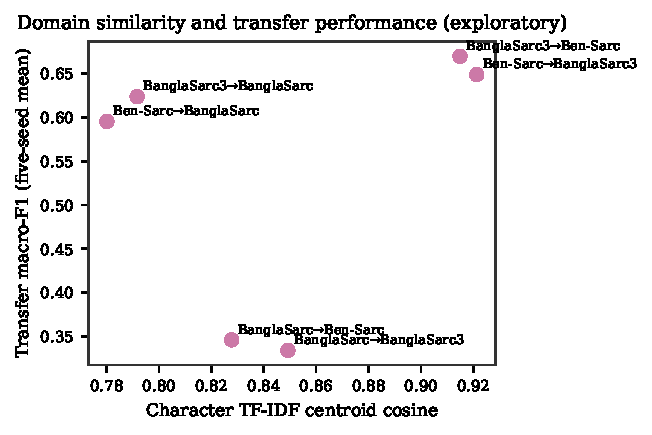
\includegraphics[width=0.48\textwidth]{F18_shift_vs_transfer}\hfill
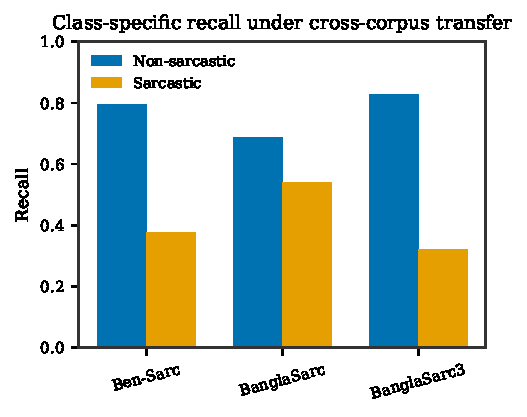
\includegraphics[width=0.42\textwidth]{F18_transfer_recall_asymmetry}
\caption{Exploratory transfer diagnostics. Left: character TF--IDF centroid cosine similarity versus five-seed mean transfer macro-F1 over six directed cells; Spearman $\rho=0.43$, $p=0.40$. Right: class-recall asymmetry for FGM transfer cells, including near-total sarcastic-class collapse when BanglaSarc is the source.}
\label{fig:shift-transfer}
\end{figure*}

\subsection{Ensemble Ablation}
\label{sec:ensemble-results}

For completeness we asked what combining the trained models buys. Given $K$ fine-tuned models with probability outputs $\hat{p}^{(k)}$, soft voting averages them, $\bar{p}_c = \tfrac{1}{K}\sum_k \hat{p}^{(k)}_c$, while stacking fits a logistic-regression meta-learner on the concatenated validation probabilities,
\begin{equation}
\hat{p}^{\mathrm{stack}} = \mathrm{softmax}\!\big(\mathbf{W}_m\big[\hat{p}^{(1)}\Vert\cdots\Vert\hat{p}^{(K)}\big] + \mathbf{b}_m\big),
\label{eq:stacking}
\end{equation}
with $\mathbf{W}_m$ and $\mathbf{b}_m$ trained on validation predictions so the meta-learner never sees test data.

Results are in \cref{tab:ensemble}. Stacking gives the largest observed macro-F1, 0.8115, or $+0.0077$ over the exploratory enhanced run. McNemar gives $\chi^2=2.56$ and $p=0.1093$ for paired correctness. Because a paired-bootstrap macro-F1 comparison was not saved, this result supports only the narrower statement that an accuracy difference was not detected by McNemar; it does not establish that the macro-F1 difference is nonsignificant. The ensemble also requires multiple models at inference.

\begin{table}[!t]
\centering
\caption{Single-run ensemble ablation on \dset{Ben-Sarc} binary. $\Delta$ is relative to the exploratory enhanced run (0.8038). Only stacking was compared by McNemar on paired correctness ($p=0.1093$); no direct paired macro-F1 test is available.}
\label{tab:ensemble}
\footnotesize
\setlength{\tabcolsep}{2pt}
\begin{tabular}{@{}lcc@{}}
\toprule
\textbf{Ensemble} & \textbf{Test macro-F1} & \textbf{Difference vs.\ best single} \\
\midrule
Stacking (LR) & \textbf{0.8115} & $+0.0077$ \\
Soft vote (all) & 0.8091 & $+0.0053$ \\
Hard vote (all) & 0.8091 & $+0.0053$ \\
Soft vote (top-5) & 0.8006 & $-0.0032$ \\
Soft vote (top-3) & 0.7983 & $-0.0055$ \\
\bottomrule
\end{tabular}
\end{table}

\subsection{Head-to-Head Against the Reproduced Reference Paper}
\label{sec:headtohead-results}

\Cref{tab:headtohead} compares the exploratory enhanced run with the strongest reproducible frozen-encoder baseline on the identical fixed Ben-Sarc test split. The paired result applies only to the evaluated substitute checkpoint. We do not extrapolate a McNemar statistic to the withdrawn checkpoint because its item-level predictions are unavailable.

\begin{table}[!t]
\centering
\caption{Same-split head-to-head on \dset{Ben-Sarc} binary. The enhanced model is one exploratory seed-42 run; it is not the five-seed configuration in \cref{tab:multiseed}. The baseline is the available frozen Bengali-BERT substitute.}
\label{tab:headtohead}
\footnotesize
\setlength{\tabcolsep}{2pt}
\begin{tabular}{@{}lccr@{}}
\toprule
\textbf{Metric} & \textbf{Enhanced} & \textbf{Frozen sub.} & \textbf{Difference} \\
\midrule
Accuracy & \textbf{80.41} & 74.44 & $+5.97$ \\
Macro precision & \textbf{80.61} & 74.45 & $+6.16$ \\
Macro recall & \textbf{80.42} & 74.44 & $+5.98$ \\
Macro F1 & \textbf{80.38} & 74.44 & $+5.94$ \\
\bottomrule
\end{tabular}
\end{table}

\subsection{Calibration, Length, and Error Analysis}
\label{sec:calibration-results}

Notebook 18 extends calibration from one saved run to all 90 repeated evaluations. For every trained source model and seed, one positive temperature is fitted on that source's validation logits and then applied unchanged to each target. On the FGM diagonals, mean raw ECE ranges from 0.0140 to 0.0758 and temperature scaling lowers it for all three corpora (\cref{tab:calibration-primary}). The corresponding Brier score also decreases in every row. Averaged across the three diagonal cells, FGM ECE falls from 0.0446 to 0.0234; across the six shifted cells it falls from 0.2734 to 0.2470. Vanilla shows the same pattern, 0.0591 to 0.0289 in-domain and 0.2853 to 0.2479 cross-corpus (\cref{fig:cross-domain-calibration}). Calibration therefore degrades sharply under shift, and source-validation temperature scaling helps but does not remove the problem.

\begin{table*}[!t]
\centering
\caption{Five-seed mean calibration of the FGM system on in-domain cells. Temperature is fitted only on the corresponding source validation split. Lower is better.}
\label{tab:calibration-primary}
\small
\setlength{\tabcolsep}{5pt}
\begin{tabular}{@{}lccccc@{}}
\toprule
\textbf{Corpus} & \textbf{Raw ECE} & \textbf{Scaled ECE} & \textbf{Raw Brier} & \textbf{Scaled Brier} & \textbf{Macro-F1} \\
\midrule
Ben-Sarc & 0.0439 & 0.0215 & 0.2905 & 0.2830 & 0.7984 \\
BanglaSarc & 0.0140 & 0.0107 & 0.0292 & 0.0283 & 0.9817 \\
BanglaSarc3 & 0.0758 & 0.0380 & 0.3378 & 0.3251 & 0.7595 \\
\bottomrule
\end{tabular}
\end{table*}

\begin{figure*}[!t]
\centering
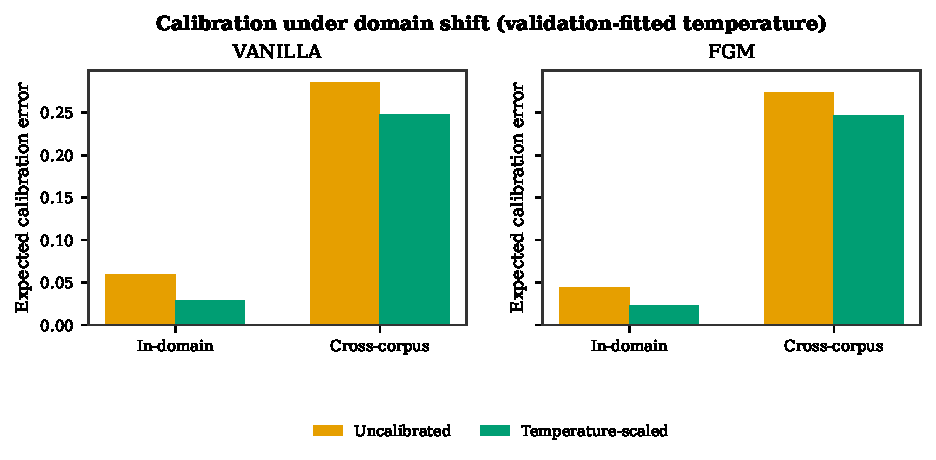
\includegraphics[width=0.80\textwidth]{F18_cross_domain_calibration}
\caption{Mean ECE before and after source-validation temperature scaling, aggregated separately over diagonal and off-diagonal cells. Shifted predictions remain substantially less calibrated for both systems.}
\label{fig:cross-domain-calibration}
\end{figure*}

\Cref{tab:calibration} preserves the earlier exploratory configuration comparison rather than discarding it. Raw ECE is 0.0219 for the enhanced run and 0.0550 for its saved vanilla baseline; after validation-fitted scaling they become 0.0210 and 0.0192. Because these configurations differ in head, sequence length, schedule, label smoothing, and adversarial procedure, the comparison does not isolate the cause. ECE is also bin-dependent, so it is reported with the 15-bin definition and Brier score rather than as a standalone deployment guarantee.

\begin{table*}[!t]
\centering
\caption{Supporting single-run calibration on Ben-Sarc with $M\!=\!15$ ECE bins. This earlier configuration comparison is not the repeated analysis in \cref{tab:calibration-primary}.}
\label{tab:calibration}
\small
\setlength{\tabcolsep}{3.5pt}
\begin{tabular}{@{}lccccc@{}}
\toprule
\textbf{Model} & \textbf{macro-F1} & \textbf{ECE} & \textbf{Brier} & \textbf{Temperature} & \textbf{Scaled ECE} \\
\midrule
Enhanced (single run) & \textbf{0.8038} & \textbf{0.0219} & \textbf{0.2791} & 0.96 & 0.0210 \\
Vanilla (hard targets) & 0.8025 & 0.0550 & 0.2884 & 1.33 & \textbf{0.0192} \\
\bottomrule
\end{tabular}
\end{table*}

Stratifying the enhanced run by comment length gives accuracy 0.787 for 0--40 characters, 0.854 for 120--200, and 0.782 for the longest bin. These are descriptive subgroup results; they do not establish why the bins differ.

The enhanced run's confusion matrix is $\left[\begin{smallmatrix}1081&200\\302&980\end{smallmatrix}\right]$, with rows and columns ordered as non-sarcastic then sarcastic, giving 302 false negatives and 200 false positives. Inspection of its most confident errors suggests that some sarcastic items use surface-sincere praise, condolences, greetings, or prayers. This qualitative observation motivates context-aware follow-up work but does not prove that the required context is absent from every item.

\subsection{Negative Results and Reproduction Faithfulness}
\label{sec:negative-results}

The reproduction is protocol-faithful rather than bit-exact: the original Ben-Sarc split was unavailable, and the strongest Indic-Transformers checkpoint could not be retrieved. The available Bengali-BERT substitute is therefore labelled explicitly in every comparison. Claims are limited to models whose predictions were evaluated on the shared split; no hypothetical adjustment is made for the withdrawn model.

\section{Discussion}
\label{sec:discussion}

\subsection{What Actually Moves the Needle}
\label{sec:discussion-win}

The most defensible modeling result is the gap between the available frozen-encoder reproduction (0.7444 macro-F1) and end-to-end fine-tuning. The older saved vanilla run reaches 0.8025, while the final native-head five-seed means are 0.7914 for vanilla and 0.7984 for FGM. The enhanced single run is not separated from its saved vanilla comparator. The five-seed exact tests cannot resolve small FGM effects, and the positive BanglaSarc-diagonal parametric interval should motivate a higher-seed confirmatory experiment rather than a claim of either superiority or equivalence. AWP is worse in the tested single-seed ablation. These observations do not invalidate earlier papers, whose pipelines and splits differ; they delimit what the evaluated implementations and frozen split support.

The calibration evidence now has two levels. The repeated native-head analysis shows that validation-fitted temperature scaling improves mean ECE and Brier score on all three diagonals, but cross-corpus ECE remains high. The older enhanced-versus-vanilla comparison remains configuration-level because multiple components change simultaneously; an isolated ablation would be required for causal attribution.

\subsection{Cross-Corpus Generalization}
\label{sec:discussion-deployment}

The repeated cross-corpus matrix is the central contribution. For FGM, the
three row-wise gaps range from 0.1126 to 0.6416, and mean off-diagonal macro-F1
is 0.5364 versus 0.8465 in-domain. Because row-wise gaps confound source and
target difficulty, the fixed-target sensitivity is more diagnostic: FGM
retains only 0.433--0.851 of the corresponding target-trained macro-F1 across
directed pairs, and vanilla retains 0.438--0.844. Every one of the 12
unadjusted, fixed-split descriptive intervals of seed-wise paired loss in
\cref{tab:fixed-target} is above zero. The same qualitative degradation appears
for both systems on source-independent target populations, but these intervals
are not simultaneous confirmatory tests.

The observed cross-corpus degradation is not a clean decomposition of pure covariate shift. Platform, topic, collection period, sampling procedure, annotation instructions, and negative-class policy move together across the three releases. The six-pair lexical audit documents that the evaluation environments differ but cannot assign a causal share to any factor. In particular, dropping BanglaSarc3 neutral items constructs an explicit binary contrast that need not coincide with the originally binary corpora's treatment of ambiguous or neutral-like comments. We therefore avoid claims that the model alone causes the entire loss or that one numeric label denotes an identical construct everywhere.

This study diagnoses the failure rather than evaluating a remedy. Pooled multi-corpus training, leave-one-corpus-out training, source balancing, and domain adaptation would change the research question from ``does a source-only model transfer?'' to ``which additional target diversity mitigates the loss?'' Mixing those protocols into the source-only matrix would obscure the deployment baseline being measured. They are important next experiments, but their absence does not alter the observed source-only degradation. The actionable conclusion supported here is narrower: source-only in-domain validation is insufficient, and a deployment claim requires evaluation on a target-representative sample.

\subsection{Limitations}
\label{sec:discussion-limitations}

\runin{Construct validity.} Macro-F1 gives both binary classes equal weight and is appropriate for the imbalanced BanglaSarc task, but it does not measure every deployment cost. We therefore report class recall, calibration, accuracy, and Brier score where saved probabilities permit them. More importantly, a shared numeric label does not guarantee a shared construct. BanglaSarc3 neutral items are dropped rather than merged, while the originally binary corpora may encode ambiguity or neutrality within their negative class. Annotation instructions, annotator populations, and platform sampling therefore remain inseparable from measured corpus shift. We did not run neutral-merged or ternary cross-corpus sensitivity analyses because compatible labels are unavailable in the other corpora. The comments also lack conversational history, speaker identity, images, prosody, and annotator disagreement; an apparent error may reflect genuine ambiguity or missing context.

\runin{Internal validity.} The primary vanilla and FGM systems share the same splits, seeds, optimizer, and evaluation code, and every transfer target is filtered against the full source corpus. This controls the principal comparisons, but it cannot rule out undetected semantic or template-level near-duplicates because the audit uses normalized exact matching. The fixed target populations are computed from the split keys rather than from prediction-file availability, and an independent prediction-file intersection recovers exactly the same 2{,}563, 436, and 762 items. An older classical cross-corpus output used a weaker train-only overlap rule and is consequently excluded from comparative evidence. The enhanced-head run changes pooling, sequence length, schedule, label smoothing, and adversarial procedure simultaneously, so it remains a configuration comparison rather than a component ablation. Likewise, the strongest frozen checkpoint from the reference study was unavailable; its clearly named substitute prevents a direct reproduction claim. Validation data determine checkpoint and temperature selection, yet repeated inspection of the same corpora during project development may still create researcher-level adaptation that is not captured by the train/test boundary.

\runin{Conclusion validity.} Five seeds improve on a selected single run but remain a small sample. The exact sign-flip test has only $2^5$ assignments and a minimum two-sided raw $p$-value of 0.0625, so nonsignificance was unavoidable at the 0.05 level even before Holm correction. The result must be read as unresolved, not as evidence of equivalence or a zero FGM effect. Student-$t$ intervals quantify training-seed variation under parametric assumptions, while item-bootstrap intervals quantify test-item variation for a fixed model. Neither captures split-selection uncertainty or uncertainty from drawing new corpora, platforms, or annotation teams. All primary estimates are conditional on one frozen split, and the single-run supporting experiments must not be read as repeated estimates.

\runin{External validity.} Transfer covers three Bengali social-media corpora and one fixed split per corpus. Conservative all-source overlap filtering changes two target sizes; the dataset-defined fixed-target sensitivity removes that row-comparison confound but does not remove semantic near-duplicates or label-policy differences. The shift association has only six directed observations and cannot rank causal sources of degradation. The study neither tests mitigation nor establishes robustness to other languages, genres, time periods, or moderation policies. Its estimates should be read as conditional on these corpora and their frozen partitions, not as a population-wide Bengali performance guarantee.

\section{Conclusion and Future Work}
\label{sec:conclusion}

This work reassesses Bengali sarcasm detection through auditable normalized-key splitting, same-split reproduction, matched tests, repeated-seed reporting, and cross-corpus evaluation. On Ben-Sarc, the primary native-head FGM system obtains $0.7984\pm0.0035$ macro-F1 over five seeds versus $0.7914\pm0.0085$ for vanilla. Five seeds are insufficient for the prespecified exact test to attain $p<0.05$, so the study cannot resolve a small FGM effect and does not claim equivalence. A separate enhanced run obtains 0.8038 but is not separated from its saved vanilla comparator under paired bootstrap. End-to-end fine-tuning materially exceeds the available frozen-encoder reproduction. The transfer gap dominates: FGM mean cross-corpus macro-F1 is 0.5364 compared with 0.8465 in-domain. On dataset-defined fixed targets, FGM retains only 0.433--0.851 and vanilla only 0.438--0.844 of target-trained macro-F1; all 12 paired-loss intervals are above zero. This is consistent evidence of substantial cross-corpus degradation on the evaluated frozen splits, not proof that a single model-side mechanism explains the loss.

These results favor evaluation improvements over a new-architecture claim. Future work should test pooled and leave-one-corpus-out training, source balancing, and domain adaptation with repeated seeds; measure semantic near-duplicate leakage; audit a blinded cross-corpus sample under one annotation guideline; preserve annotator disagreement; and add conversational or multimodal context. Any deployment claim should include target-domain validation rather than relying on a single in-domain score.

\makeatletter
\let\@texttop\relax
\def\@textbottom{\vskip\z@\@plus 1fill}
\makeatother

\phantomsection
\section*{Ethics and Data Governance}
\addcontentsline{toc}{section}{Ethics and Data Governance}
This secondary analysis used only the text and labels distributed with previously published social-media datasets; it involved no new recruitment, interaction, intervention, identifier collection, or re-identification. The reported experiments were executed on local copies, and the public repository contains only hashed keys and numerical artifacts, with no comment text or reversible normalized strings. Ben-Sarc is distributed for non-commercial research under CC BY-NC-SA 4.0 \cite{bensarcRepository}, while BanglaSarc3 is published under CC BY 4.0 \cite{banglasarc3Mendeley}. Because a separately verifiable license statement for the BanglaSarc archive was not present in the project record, no BanglaSarc text is redistributed; researchers must obtain every source corpus from its publisher and comply with the applicable terms and institutional requirements. The article reports no third-party prompted-API experiment, thereby avoiding a claim that dataset licenses authorized transmission of comments to an external model provider.

\phantomsection
\section*{Data and Code Availability}
\addcontentsline{toc}{section}{Data and Code Availability}
All code, Notebook 18, the long-form 90-cell record, the 90 text-free prediction files, nine hashed split manifests, fixed-target uncertainty tables, paired tests, and the configuration and audit files listed in \cref{tab:provenance-map} are available in the public repository at \url{https://github.com/Sefayet-Alam/Beyond_In_domain_Bangla_Sarcasm_Detection}. Reviewers should use the tagged release, which is the single source of reproduction: its \path{04_outputs/finalized_outputs/MANIFEST_sha.json} inventory carries per-file SHA-256 hashes, so any downloaded artifact can be checked against the manuscript with no separate archive or supplement. Source corpora are not redistributed and remain subject to their original terms. A DOI-backed archival deposit of the tagged release will accompany the version of record.

\phantomsection
\section*{Acknowledgment}
\addcontentsline{toc}{section}{Acknowledgment}
The authors used AI writing assistants---Anthropic Claude \cite{anthropicClaude}, OpenAI ChatGPT \cite{openaiChatGPT}, and QuillBot QuillBot \cite{quillbot} ---only to improve language and check grammar. Their role was limited to wording, phrasing, and proofreading. They did not design the study, select data, run experiments, analyze results, or draw conclusions, and they do not qualify for authorship. Every figure, table, and number in this paper comes from the authors' own code and experiments, and the authors take full responsibility for the content.

\phantomsection
\bibliographystyle{IEEEtran}
\bibliography{references}

\begin{IEEEbiography}[{
\includegraphics[width=1in,height=1.25in,clip,keepaspectratio]{author_alam.png}}]{Khandoker Sefayet Alam}
is currently pursuing the B.Sc.\ degree in computer science and engineering with the Rajshahi University of Engineering and Technology (RUET), Rajshahi, Bangladesh.

In 2025 he completed an industrial attachment with Vivasoft Limited, Dhaka, Bangladesh, working on full-stack web development, and he has previously worked under contract evaluating the outputs of code-generation models. His research interests include natural language processing for low-resource languages, reproducible machine-learning evaluation, and cross-corpus generalization.

Mr.\ Alam competed in the ICPC Asia Dhaka Regional Contest in 2024 and 2025, and placed eighth among more than 120 teams at the UIU Inter-University Programming Contest in 2025.
\end{IEEEbiography}

\begin{IEEEbiography}[{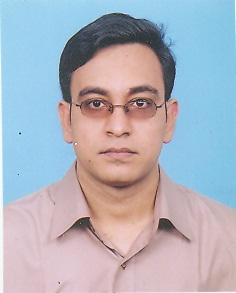
\includegraphics[width=1in,height=1.25in,clip,keepaspectratio]{author_islam.png}}]{Md. Rabiul Islam}
received the Ph.D.\ degree from the Department of Electrical and Electronic Engineering, Rajshahi University of Engineering and Technology (RUET), Rajshahi, Bangladesh, in 2012.

He is currently a Professor with the Department of Computer Science and Engineering, RUET, and the Director of its Institute of Information and Communication Technology (IICT). He has served as the Dean of the Faculty of Electrical and Computer Engineering, RUET. A long strand of his work applies machine learning to bioinformatics, recovering interpretable structure from large-scale biological data. His research interests include biomedical engineering, pattern recognition, deep learning, and biometrics.
\end{IEEEbiography}

\begin{IEEEbiography}[{
\includegraphics[width=1in,height=1.25in,clip,keepaspectratio]{author_ahamed.png}}]{Md. Faysal Ahamed}
received the B.Sc.\ degree in electrical and computer engineering from the Rajshahi University of Engineering and Technology (RUET), Rajshahi, Bangladesh, in 2022, ranking second in his department, and subsequently completed the M.Sc.\ degree in computer science and engineering.

He joined RUET as a Lecturer with the Department of Electrical and Computer Engineering in January 2024, and has been an Assistant Professor there since September 2025. He has authored or co-authored 26 journal articles, 13 conference papers, and nine books and book chapters, and has collaborated with the Machine Learning Laboratory, Qatar University. His research interests include medical image processing, image classification, segmentation, and localization, and the design of efficient deep-learning models with explainable artificial intelligence.

Mr.\ Ahamed was a recipient of the Excellent Research Award from the Department of Electrical and Computer Engineering, RUET, in 2022, and the Student of the Year Award in 2021 and 2022.
\end{IEEEbiography}

\begin{IEEEbiography}[{
\includegraphics[width=1in,height=1.25in,clip,keepaspectratio]{author_chowdhury.png}}]{Muhammad E. H. Chowdhury}
(Senior Member, IEEE) received the Ph.D.\ degree in electrical engineering from the University of Nottingham, Nottingham, U.K., in 2014.

He was a Postdoctoral Research Fellow with the Sir Peter Mansfield Imaging Centre, University of Nottingham. He is currently an Assistant Professor and the Program Coordinator with the Department of Electrical Engineering, Qatar University, Doha, Qatar. He holds several patents and has authored or co-authored more than 250 peer-reviewed journal articles, over 30 conference papers, and three edited books. His research interests include biomedical instrumentation, signal processing, wearable sensors, medical image analysis, machine learning and computer vision, embedded system design, and simultaneous EEG/fMRI.

Dr.\ Chowdhury serves as an Associate Editor for \emph{Computers and Electrical Engineering} and IEEE Access. He was a recipient of the COVID-19 Dataset Award in 2020 and is listed among the top 2\% of scientists worldwide.
\end{IEEEbiography}

\EOD

\end{document}